%%
%% Copyright 2007-2024 Elsevier Ltd
%%
%% This file is part of the 'Elsarticle Bundle'.
%% ---------------------------------------------
%%
%% It may be distributed under the conditions of the LaTeX Project Public
%% License, either version 1.3 of this license or (at your option) any
%% later version.  The latest version of this license is in
%%    http://www.latex-project.org/lppl.txt
%% and version 1.3 or later is part of all distributions of LaTeX
%% version 1999/12/01 or later.
%%
%% The list of all files belonging to the 'Elsarticle Bundle' is
%% given in the file `manifest.txt'.
%%
%% Template article for Elsevier's document class `elsarticle'
%% with numbered style bibliographic references
%% SP 2008/03/01
%% $Id: elsarticle-template-num.tex 249 2024-04-06 10:51:24Z rishi $
%%
% =============================================================================
%  UPDATED AGAINST THE RUNS OF 2026-08-14
%
%  Regenerated sources used for every number below:
%     tex/tables/{gap,gap_nopen,feasibility,runtime}.tex          (2026-08-14 10:04)
%     tex/tables/additional_{diesel,diesel_decomp,diesel_refuel,
%                            diesel_tw,la,la_policy,sensitivity,vss}.tex (10:07-10:21)
%     data_output/{paper_gap_stats,additional_sens_stats,
%                  additional_diesel_stats,additional_la_stats}.csv
%     figures/*.png  (2026-08-14)
%
%  COLOUR CONVENTION FOR THIS REVISION
%     \red{...}    = changed by me against the previous draft (new numbers,
%                    rewritten claims, retired claims)
%     \blue{...}   = still needs the runs that are not on disk yet
%     \green{...}  = my comment to you, to be deleted before submission
% =============================================================================
\documentclass[preprint,12pt,3p]{elsarticle}

%% Use the option review to obtain double line spacing
%% \documentclass[authoryear,preprint,review,12pt]{elsarticle}

%% Use the options 1p,twocolumn; 3p; 3p,twocolumn; 5p; or 5p,twocolumn
%% for a journal layout:
%% \documentclass[final,1p,times]{elsarticle}
%% \documentclass[final,1p,times,twocolumn]{elsarticle}
%% \documentclass[final,3p,times]{elsarticle}
%% \documentclass[final,3p,times,twocolumn]{elsarticle}
%% \documentclass[final,5p,times]{elsarticle}
%% \documentclass[final,5p,times,twocolumn]{elsarticle}

%% For including figures, graphicx.sty has been loaded in
%% elsarticle.cls. If you prefer to use the old commands
%% please give \usepackage{epsfig}

\usepackage{amssymb}
\usepackage{amsmath}
\usepackage{comment}
\usepackage{natbib}
\usepackage{doi}
\usepackage{xcolor}
\usepackage{enumitem}
\usepackage{multirow}

\bibliographystyle{plainnat}
\usepackage{booktabs}
\usepackage{subcaption}
%% \usepackage{amsthm}
\usepackage{amsmath}

\newcommand{\red}[1]{\textcolor{red}{#1}}
\newcommand{\black}[1]{\textcolor{black}{#1}}
\newcommand{\orange}[1]{\textcolor{orange}{#1}}
\newcommand{\purple}[1]{\textcolor{purple}{#1}}
\definecolor{darkgreen}{rgb}{0.0, 0.3, 0.0}
\newcommand{\green}[1]{{\color{darkgreen}#1}}
% -- added for this revision: \blue{} marks what still needs runs
\definecolor{darkblue}{rgb}{0.0, 0.0, 0.7}
\newcommand{\blue}[1]{{\color{darkblue}#1}}


%% The lineno packages adds line numbers. Start line numbering with
%% \begin{linenumbers}, end it with \end{linenumbers}. Or switch it on
%% for the whole article with \linenumbers.
%% \usepackage{lineno}
\begin{comment}
\journal{Energy}
\end{comment}
\begin{document}

\begin{frontmatter}

%% Title, authors and addresses

%% use the tnoteref command within \title for footnotes;
%% use the tnotetext command for theassociated footnote;
%% use the fnref command within \author or \address for footnotes;
%% use the fntext command for theassociated footnote;
%% use the corref command within \author for corresponding author footnotes;
%% use the cortext command for theassociated footnote;
%% use the ead command for the email address,
%% and the form \ead[url] for the home page:
%\title{Title\tnoteref{label1}}
%\tnotetext[label1]{Corresponding author}
%\author{Céline V. Pagnier}
%\ead{celine.pagnier@ntnu.no}
%\ead[url]{home page}
\fntext[label2]{Corresponding author: celine.pagnier@ntnu.no}
%\cortext[cor1]{Corresponding author: celine.pagnier@ntnu.no}
%% \affiliation{organization={},
%%             addressline={},
%%             city={},
%%             postcode={},
%%             state={},
%%             country={}}
%\fntext[label3]{}

\title{Joint scheduling of driver activities and charging for long distance electric truck operation under travel time uncertainty}



\author[inst1, label1]{Céline Pagnier}
\author[inst2]{Margaux Nattaf}
\author[inst2]{Marie-Laure Espinouse}
\author[inst3]{Cyrille Briand}
\author[inst1]{Steffen J.S. Bakker}


\affiliation[inst1]{organization={Department of Industrial Economics and Technology Management, Norwegian University of Science and
Technology},%Department and Organization
            addressline={Alfred Getz veg 3},
            city={Trondheim},
            postcode={NO-7491},
            %state={State One},
            country={Norway}}
\affiliation[inst2]{organization={Univ. Grenoble Alpes, CNRS, Institute of Engineering Univ. Grenoble Alpes, G-SCOP},%Department and Organization
            %addressline={Instituttveien 18, 2007 Kjeller},
            city={Grenoble},
            postcode={38000},
            %state={State Two},
            country={France}}

\affiliation[inst3]{organization={LAAS-CNRS, Université	de	Toulouse, CNRS,	UT3},%Department and Organization
            %addressline={Instituttveien 18, 2007 Kjeller},
            city={Toulouse},
            postcode={31000},
            %state={State Two},
            country={France}}


%\begin{comment}

%% Abstract
\begin{abstract}
Battery electric trucks are entering long-haul freight operations, but various additional constraints compared to conventional diesel trucks discourage freight companies from transitioning their fleets.
As charging infrastructure expands, long-haul routes become increasingly feasible, and efficient schedules seek to synchronize charging stops with mandatory driver breaks. However, this synchronization remains fragile due to battery limitations and operational uncertainty, and becoming stranded due to lack of battery is unacceptable.
This paper studies the joint scheduling of driver activities, such as breaks and rests, and partial non-linear fast charging activities for a battery electric truck serving a fixed sequence of customers on a long-haul route under travel-time uncertainty.

We formulate a mixed-integer linear program capturing the Hours of Service regulations, including split breaks, reduced rests, extended driving allowances, and the interaction between charging and break. Around this model, we build and compare six decision architectures that differ in when decisions are committed and what information they use: a scenario-based rolling-horizon look-ahead policy, a myopic greedy policy, a robust plan, a budgeted robust plan, a two-stage stochastic plan with online duration recourse, and a perfect-hindsight oracle.

\red{Experiments on 450 corridor instances show that the decision architecture, and not the sophistication of the policy, is what separates the methods: the two online policies and the two-stage plan all land within 3--12\,\% of the perfect-hindsight optimum, whereas plans whose durations are committed at departure against a worst case lose 28--35\,\%.}
\red{Electrifying these corridors costs 8--10\,\% of route duration against a diesel truck on identical routes and identical travel-time realizations, rising to only 12\,\% for an operator scheduling myopically, so roughly a quarter of the observed electrification penalty is a planning failure and the remainder is a physical cost that better scheduling cannot remove.}
\red{Finally, decision makers should direct charging-infrastructure investment towards more powerful chargers rather than a denser network: at the spacing already mandated by Regulation (EU) 2023/1804, charger power outweighs charger density by a factor of roughly four in route duration reduction, and the asymmetry is sharper still downwards, a 150\,kW corridor costing 19\,\% of route duration against the 1.5\,\% cost of thinning the network from 60 to 100\,km. This shifts the burden onto grid connection capacity at each site.}

\end{abstract}

\green{Comment on the abstract: the two headline numbers that moved most are the
myopic electrification penalty (was 20--23\,\%, now 12\,\%) and the greedy gap to
oracle (was 21/19/14\,\%, now 8/7/6\,\%). Both follow from the same change in the
greedy policy, so the "roughly half of the penalty is a planning failure"
sentence of the previous draft is no longer supported and has been retired.}


%% Keywords
\begin{keyword}
%% keywords here, in the form: keyword \sep keyword
Electric trucks \sep TDSP \sep travel time uncertainty \sep rolling horizon
\end{keyword}

\end{frontmatter}

%% Add \usepackage{lineno} before \begin{document} and uncomment
%% following line to enable line numbers
%% \linenumbers





\section{Introduction} \label{intro}
Road freight accounts for roughly a quarter of transport $CO_2$ emissions in the European Union, and battery electric heavy-duty trucks (BEHDTs) are the leading decarbonization pathway for the segment. Their deployment in long-haul  service, however, is first constrained by battery capacity and charging infrastructure, but also by an operational factor that is absent for passenger electric vehicles: driver's regulations. Commercial drivers in the EU operate under Regulation (EC) No 561/2006 and Directive 2002/15/EC, which impose mandatory breaks after at most 4.5 h of driving, daily rest periods, and limits on shift driving time.
Because a mandatory 45-minute break is long enough for a substantial fast charge, synchronization of charging and drivers constraints is critical. Whether electric long-haul operation can match diesel route durations therefore hinges on how well charging events can be synchronized with legally required interruptions.

However, this synchronization is fragile. Travel times on long-haul corridors are uncertain, and a delay on a single leg propagates through the entire schedule: it consumes driving-time budget before the planned break location is reached, shifts arrivals outside customer service windows, and, because energy consumption depends on realized speed, perturbs the state of charge with which the truck reaches the next charging opportunity. A pre-determined schedule that nests charging inside breaks under average travel times may, in execution, force
the driver into an unacceptable event such as running out of battery if the energy consumption deviates from anticipated values.

This paper studies the joint scheduling of driver activities and charging for a battery electric truck on a fixed long-haul route with multiple customer stops, under stochastic travel times. Given the sequence of customers, the decisions are where and for how long to charge (with a nonlinear, piecewise-linearized charging curve and partial charging), where to take breaks and daily rests (including split breaks, reduced rests, and extended driving allowances, together with the rule that a sufficiently long charging stop can count as a break), so as to minimize route duration while respecting the daily provisions of EU HoS regulation, battery limits, and customer service windows.


Because decisions are taken sequentially while uncertainty is revealed leg by leg, the central methodological question is about the decision architecture: when should each decision be committed, and what information should it use? We organize our solution methods along exactly this axis. Three offline methods that commit a plan before departure: a box robust plan over an interval uncertainty set, a budgeted robust plan that protects only against a bounded number of simultaneous worst-case legs, and a two-stage stochastic plan whose activity structure is fixed but whose durations adapt online, and two online architectures that re-decide at every stop: a scenario-based rolling-horizon look-ahead policy and a myopic greedy policy representing typical driver behavior. All methods are evaluated in a common discrete-event simulation, and benchmarked against a perfect-hindsight oracle, so that the value of information and the value of adaptivity can be measured directly.


Our contributions are as follows.
First, we model the full weekly provisions of the EU Hours-of-Service (HoS) regulation in the context of electric trucks, incorporating partial charging along a non-linear charging curve. We formulate this as a MILP and validate it against an independent exact method for the HoS rules.
Second, we analyze the impact of travel-time uncertainty through an extensive set of methods spanning different decision architectures, quantifying the effect of committing to a schedule upfront versus adapting en route as new information is revealed.
Third, we quantify the electrification penalty of long-haul routes by decomposing it into charging time, additional station-access time. This corroborates the finding of \citet{brockmann_break-and-charge_2025} that mandatory breaks provide sufficient charging windows most of the time, with charge/break coupling of \red{70--76\,\%}, while showing that the access overheads of a fast-charging stop, which that work does not consider, \red{absorb roughly a third of the resulting credit}.
Finally, we derive policy insights regarding charging-infrastructure investment along long-haul corridors. In particular, that charger power outweighs charger density by a factor of roughly four in its effect on route duration.
\red{We additionally report a battery-capacity axis, which the previous draft did not cover, and a real-life case study reconstructed from the telematics of a six-day international tour.}


The remainder of the paper is organized as follows. Section \ref{sec:litreview} reviews related work. Section \ref{sec:problem_definition} defines the problem and states the modeling assumptions. Section \ref{sec:model} presents the deterministic MILP. Section \ref{sec:method} describes the simulation framework and the {six} decision architectures. Section \ref{sec:exp} details the experimental design, and Section \ref{sec:results} reports the computational results \red{and discusses their implications}. Section \ref{section:conclusion} concludes.
\green{(The previous draft pointed at a \texttt{sec:discussion} label that does not exist, which rendered as ``Section ??''. There is no separate discussion section, so I folded the clause into the results sentence.)}



%%%%%%%%%%%%%%%%%%%%%%%%%%%%%%%%%%%%%%%%%%% -------------------------------------------------------------------------------


\section{Literature review} \label{sec:litreview}
\subsection{The truck driver scheduling problem}
Hours-of-service (HoS) regulations impose constraints on the working and driving schedule of commercial vehicle drivers. In the European Union, Regulation~(EC) No~561/2006 \citep{noauthor_regulation_2006} specifies maximum consecutive and daily driving times, mandatory break structure and minimum daily rest periods. A similar directive (2002/15/EC) limits total shift working time and restricts work during night hours. Together these rules define the truck driver scheduling problem (TDSP): given a fixed sequence of customer stops, find a feasible and cost-efficient driver schedule complying with all regulatory constraints.


The first work to model government HoS constraints in a scheduling context is \citet{xu_solving_2003}, who study a rich pickup-and-delivery problem under US rules and conjecture that finding a minimum-cost compliant schedule is NP-hard with multiple time windows. \citet{archetti_trip_2009} show that the US TDSP with single time windows is solvable in $O(n^3)$ time. For European rules, \citet{drexl_labelling_2010} formalize EU HoS as resource constraints in the elementary shortest path problem with resource constraints (ESPPRC), develop exact and heuristic labeling algorithms, and conjecture NP-completeness. \citet{goel_vehicle_2009} proposes a depth-first label-setting procedure for EU rules, which is extended in \citet{goel_truck_2010} to cover extended driving allowances and reduced rest exceptions. \citet{kok_dynamic_2010} present a dynamic programming heuristic for combined vehicle routing and driver scheduling under full EU social legislation, showing that the flexibility of complex break rules yields substantial cost reductions. \citet{prescott-gagnon_european_2010} embed EU driver rules as resources in a column-generation framework for the VRP with time windows, treating the TDSP as a pricing subproblem. \citet{rancourt_long-haul_2013} address long-haul routing under US HoS with tabu search, confirming that the choice of embedded scheduling algorithm significantly impacts solution quality. \citet{goel_hours_2014} compare EU, US, Canadian and Australian HoS regulations through optimization, finding that EU rules achieve the highest road safety at a moderate cost premium. Exact branch-and-price algorithms for the combined VRTDSP are developed by \citet{goel_exact_2017}, which is the first with proven optimality guarantees. This method is subsequently accelerated by \citet{tilk_bidirectional_2020} via bidirectional labeling. The most comprehensive EU treatment to date is \citet{garaix_label-setting_2024}, who develop a label-setting algorithm for the weekly TDSP and are the first to model the night-work rule, which limits shift working time to ten hours when night work is performed. Across this literature the driver schedule is computed once, against deterministic travel times. To our knowledge no exact EU TDSP formulation has been integrated in a sequential decision framework in which uncertain leg durations are revealed as the route is executed, which is the setting of the present paper.


\subsection{The electric vehicle routing problem}
The electric vehicle routing problem (EVRP) extends classical vehicle routing to account for the limited driving range of battery electric vehicles and the need for en-route recharging at charging stations. For a comprehensive survey we refer to \citet{erdelic_survey_2019}. The foundational formulation is the green VRP of \citet{erdogan_green_2012}, which routes alternative-fuel vehicles through refueling stations with full recharging. Exact branch-price-and-cut algorithms for the EVRPTW, covering four variants from single full recharges to multiple partial recharges, are developed by \citet{desaulniers_exact_2016}, who establish that allowing both multiple and partial recharges reduces routing cost and fleet size.

Partial recharging is studied by \citet{felipe_heuristic_2014} for a multi-technology green VRP and it is shown by \citet{keskin_partial_2016} to substantially reduce route duration . Depot-level charge scheduling over multiple days, accounting for time-dependent energy prices and battery degradation, is studied by \citet{pelletier_charge_2018}. The charging function for battery follows a concave nonlinear profile due to the constant-current/constant-voltage physics of lithium-ion cells. While most work simplify this assumption by assuming a linear charging function, it may also be linearized through the use of a piecewise-linear (PWL) approximation \citep{montoya_electric_2017}.

Uncertainty at charging stations has received growing attention: \citet{keskin_simulation-based_2021} address the EVRPTW with stochastic waiting times due to limited charger availability, showing that queuing uncertainty significantly affects routing decisions. Energy consumption uncertainty is addressed by \citet{pelletier_electric_2019} using a robust optimization framework, demonstrating that robust solutions come at only a modest cost increase. The bulk of EVRP research targets light-duty vehicles in urban or regional settings. Battery electric heavy-duty trucks (BEHDTs) differ qualitatively: much larger energy demands per leg, reliance on high-power fast charging, and binding HoS constraints that govern both when the driver may be on duty and how charging time interacts with mandatory break requirements.


\subsection{Combining TDSP and EVRP}
Despite the practical importance of long-haul BET operations, the literature combining HoS regulation with battery energy management in a single optimization model is sparse. \citet{bai_rollout-based_2023} study the problem of jointly determining optimal charging and rest decisions for an electric truck on a fixed pre-planned route under HoS constraints. They formulate a bilinear MIP minimizing total cost (charging plus rest time) and develop a rollout-based approximate solver that scales linearly with the number of stations, validated on Swedish road network data.

\citet{brockmann_break-and-charge_2025} develop a mathematical programming model that synchronizes driver break times with truck charging events under EU HoS, validated on real-world data from northwest Germany. Their key finding is that mandatory breaks create natural charging windows sufficient to match diesel route durations. However they do not consider additional manever time due to access to the charging stations. \citet{wan_long-haul_2024} study long-haul truck charging planning with time and energy flexibility, proposing a mixed-integer model for opportunity charging at routine stops. \citet{su_optimizing_2025} introduce a stage-expanded graph for minimizing the carbon footprint of long-haul heavy-duty e-truck trips, simultaneously optimizing path, speed, and charging, and show that the optimized charging strategy compounds the emissions benefit of electrification. \citet{vidotte_plaza_charger_2026} are the first to jointly optimize charging infrastructure siting and HoS-compliant driver scheduling for long-haul eHDT fleets, though their focus is on strategic network design rather than operational online scheduling. Finally, \citet{niyomphon_stochastic_2026} propose a chance-constrained stochastic MILP for electric freight on fixed long-haul routes with partial recharging and uncertain freight demand, but without HoS constraints.


\subsection{Uncertainty in long-haul freight transport}
Travel time uncertainty in long-haul road freight creates two risks: a HoS violation when accumulated driving or working time exceeds its limit before a scheduled break, and battery depletion when a leg uses more energy than planned. While stochastic EVRP models have addressed energy consumption uncertainty \citep{pelletier_electric_2019} and queuing uncertainty at chargers \citep{keskin_simulation-based_2021}, travel time uncertainty and its joint effect on HoS compliance and SOC feasibility remains largely unexplored.

The framework of this type of problem where decisions have to be made sequentially, and adjusted based on realized uncertainty, fits well with the rolling horizon methodology, especially when the multi stage optimization problem would be too complex to solve. The rolling-horizon paradigm is a well-established technique for multi-period optimization under gradual information revelation \citep{glomb_rolling-horizon_2022}. The broader literature on dynamic vehicle routing \citep{pillac_review_2013} covers stochastic programming, robust optimization, and online policies, and classifies our problem as one with a fully known route structure but sequentially revealed stochastic leg costs.


\subsection{Contribution}

Table~\ref{tab:litreview} positions the present work against the most closely related papers across eight dimensions. This paper is the first to jointly model full EU HoS (including split-break sequencing, shift working-time limits, multiple rest types, and charging-break interactions), partial fast-charging with a nonlinear PWL charging curve, multiple customer stops with soft time windows on a fixed long-haul route, and stochastic travel times.

{\color{red} CHECK AGAIN TABLE}

\begin{table}[htbp]
\centering
\caption{Positioning of the present work in the literature.}
\label{tab:litreview}
\scriptsize
\setlength{\tabcolsep}{3.5pt}
\resizebox{\textwidth}{!}{%
\begin{tabular}{p{3.8cm} c p{1.8cm} p{1.5cm} c c c}
\toprule
\textbf{Reference}
  & \textbf{HoS}
  & \textbf{Charging}
  & \textbf{Route length}
  & \textbf{Fixed}
  & \textbf{TW}
  & \textbf{Uncertainty}\\
\midrule

\citealt{goel_exact_2017}   & EU & $-$ & Long-haul & $-$ & Hard & $-$\\
\citealt{garaix_label-setting_2024}   & EU & $-$ & Long-haul & $\checkmark$ & Hard & $-$\\

\citealt{montoya_electric_2017}   & $-$ & Partial + NL & Regional & $-$ & Hard & $-$\\

\citealt{keskin_simulation-based_2021}   & $-$ & Partial + L & Long-haul & $-$ & Hard & CS queues\\
\citealt{niyomphon_stochastic_2026}   & $-$ & Partial + L & Long-haul & $-$ & $-$ & Demand \\

\citealt{bai_rollout-based_2023}   & EU & Partial$+$L & Day & $\checkmark$ & $-$ & $-$\\
\citealt{brockmann_break-and-charge_2025}   & EU & Partial$+$NL  & Day & $\checkmark$ & $-$ & $-$ \\
\citealt{vidotte_plaza_charger_2026}   & Brazil & Full$+$L &  Long-haul & $-$ & Hard & $-$ \\
\midrule
This paper
  & {EU}
  & {Partial$+$NL}
  & {Long-haul}
  & $\checkmark$
  & {Soft}
  & Travel time\\
\bottomrule
\end{tabular}}
\par\smallskip
\begin{minipage}{\textwidth}
\footnotesize
\textbf{Charging}: L/NL: linear/non-linear charging function.
\textbf{TW}: customer time windows.
\end{minipage}
\end{table}


\section{Problem Definition}
\label{sec:problem_definition}

This paper studies the problem of scheduling driver activities for long-distance freight transport with a battery electric truck (BET). The schedule must simultaneously satisfy Hours-of-Service (HoS) regulations and battery energy constraints. Given a predefined sequence of customer visits, the objective is to minimize the total route duration by determining the optimal timing and locations of mandatory breaks, daily rest periods, and battery charging operations.

\subsection{Route and Customers}
The route connects a sequence of customer locations via road segments whose lengths are known in advance. Travel on each segment is characterized by an average speed. In practice, however, traffic conditions introduce uncertainty in the actual travel duration: this is explicitly accounted for in the model. The total route duration is the sum of five components: driving time accumulated while the vehicle is moving between locations, service time for loading or unloading operations, charging time at charging stations, station access and maneuvering time, and legally required interruptions such as mandatory breaks and daily rest periods.

The sequence of customers to be visited is fixed and known prior to departure. At each customer location, the driver performs a loading or unloading operation whose duration is known.
At each customer, soft time windows are considered. Service begins immediately upon arrival, whether or not the window is open: distribution terminals do not turn a truck away, but an arrival outside the announced window, either early or late, disrupts terminal planning and incurs a fixed service-level penalty, identical for early and late arrivals. Any break or rest
taken at a customer stop occurs after service. The vehicle is not permitted to wait idly for a window to open: an early arrival is served early and penalized, or the driver stretches a break at an earlier stop.

\subsection{Charging operations}
The BET has a battery of fixed capacity (kWh). Energy consumption is assumed to be dependent of the distance traveled and the vehicle speed, yielding a specific consumption rate expressed in kWh/km. At each CS stop, the driver may charge the battery either partially or fully, and multiple charging stops are permitted throughout the route. Charging is not allowed during customer service operations.

Only high-power fast charging is available along the route (overnight slow charging such as in depot is not considered). The charging process is modeled by a piecewise linear approximation of the nonlinear charge-rate curve. Queuing at a CS is modeled as a known waiting time at each CS.

Finally, a sufficiently long charging stop may simultaneously satisfy a mandatory break requirement. Specifically, a charging event counts as a driving break provided its duration meets the applicable threshold: at least 15~minutes for a first split break, at least 30~minutes for a second split break, or at least 45~minutes for a full break, as defined by the HoS regulations described below.

\subsection{HoS Regulations}
The scheduling problem is subject to European HoS regulations given by Regulation (EC) No 561/2006 (driving times, breaks and rests) and Directive 2002/15/EC (working time).
Two accumulation counters are maintained: driving time, which counts only periods when the vehicle is in motion, and working time, which additionally includes customer service, charger access and maneuvering, and charging time not covered by a simultaneous break.

Regarding mandatory breaks, a driver may not accumulate more than 4.5~hours of continuous driving without taking a full break of at least 45~minutes. This full break may be replaced by a split sequence consisting of a first period of at least 15~minutes (but less than 45~minutes) followed, in that order, by a second period of at least 30~minutes.

Regarding shift-level constraints, the maximum permitted driving time per shift is 9~hours, extendable to 10~hours on no more than two occasions per week.
%Furthermore, if the shift includes a period of night working, the total working time within that shift is limited to 10~hours.
A daily rest of at least 11 h must separate consecutive shifts, and it may be reduced to 9 h at most three times between weekly rests.
As a consequence of these rest requirements, the sum of working time, break time, and any other on-duty periods within a 24-hour window is bounded by 13~hours under a full rest, or by 15~hours when the rest is reduced to 9~hours.

Charging during rests is treated as sequential: the truck must vacate the charging bay before the rest begins, and such charging time counts as work.

While charging is only possible at charging stations,  breaks and rests may be taken at customer stops, charging stations, and dedicated rest-area nodes inserted along legs.


\section{Deterministic Mathematical Model} \label{sec:model}
We now present the mathematical formulation for the deterministic problem. Tables ~\ref{tab:notation-mini} and ~\ref{tab:notation-mini2} present all notation used in the model formulation. Figure \ref{fig:solution} present a possible solution of the problem.



\begin{table}[h!]
\centering
\caption{Notation summary.}
\label{tab:notation-mini}
\small
\begin{tabular}{p{0.12\linewidth}p{0.8\linewidth}}
\toprule
\multicolumn{2}{l}{\textbf{Sets}}\\
\midrule
$\mathcal{I}$ & Set of possible stops, ordered from 0=origin to N=destination.\\
$\mathcal{C}$ & Set of customers $\mathcal C \subseteq \mathcal I$.\\
$\mathcal{K}$ & Set of charging stations $\mathcal K \subseteq \mathcal I$.\\
$\mathcal{L}$ & Set of rest areas $\mathcal L \subseteq \mathcal I$, $\mathcal C \cap \mathcal K \cap \mathcal L= \emptyset$.\\
$\mathcal{R}$ & Set of breakpoints of the piecewise-linear charging function.\\
\midrule
\multicolumn{2}{l}{\textbf{Parameters}}\\
\midrule
$D_i$ & Travel time from stop $i$ to stop $i+1$.\\
$E_i$ & Energy consumption between stop $i$ and stop $i+1$.\\
$E^{cap}$ & Battery capacity. \\
$E^{\min}$ & Minimum SOC. \\
$E^0$ & Initial SOC. \\

$\bar{E}_r$  & SOC level at breakpoint $r \in \mathcal{R}$ of the charging fct, ($\bar{E}_0 = 0$, $\bar{E}_R = E^{cap}$).\\
$\mathcal{T}_r$ & Time to charge from empty to $\bar{E}_r$,($\mathcal{T}_0 = 0$).\\
$\mathcal{T}_{\text{min}}$ & Minimum charging time at a CS.\\


$S_i$ & Service time at customer $i \in \mathcal{C}$. \\
$Q_i$ & Queue time at CS stop $i \in \mathcal{K}$ if charging occurs. Zero if $y_i = 0$.\\
$M_i^{stop}$ & Maneuver time at CS stop $i \in \mathcal{S}$ if any activity occurs.\\
$M_i^{seq}$ & Repositioning time at stop $i \in \mathcal{K}$ when charging and a break or rest are declared sequentially, i.e. the truck must vacate the charging bay before the break begins.\\

$W_i^{Ha}, W_i^{Hf}$  & Service time window at customer $i \in \mathcal{C}$. \\
$ \beta$ & Fixed out-of-window service penalty (h). \\

%$[W_i^{Sa}, W_i^{Sf}]$  & Soft time window at customer $i \in \mathcal{C}$ \\
$T^{brk}_{b45}$   & Full break duration ($= 45$\,min). \\
$T^{brk}_{b_{15}}$     & Min first split break ($= 15$\,min). \\
$T^{brk}_{b_{30}}$     & Min second split break ($= 30$\,min). \\
$T^{rst}_{r_1}$          & Minimum daily rest duration ($= 11$\,h). \\
$T^{rst}_{r_2}$          & Reduced daily rest duration (exception 1) ($= 9$\,h at most $3\times$/week). \\
$\bar{\rho}$ & Weekly number of allowed reduced rest duration ($=3$).\\

$T^{drv}_{cons}$   & Max consecutive driving time ($= 4.5$\,h). \\
$T^{drv}_{shift_1}$     & Max shift driving time ($= 9$\,h). \\
$T^{drv}_{shift_2}$     & Increased shift driving time (exception 2) ($= 10$\,h at most $2\times$/week). \\
$\bar \epsilon $ &  Weekly number of allowed extended driving duration ($=2$).\\

$T^{wk}_{sh1}$      & Max shift working time under a regular daily rest ($= 13$\,h). \\
$T^{wk}_{sh2}$      & Max shift working time under a reduced daily rest ($= 15$\,h). \\

\bottomrule
\multicolumn{2}{l}{{\footnotesize Abbreviations: SOC = state of charge, CS = charging station}}\\
\end{tabular}
\end{table}


\begin{table}[h!]
\centering
\caption{Variables notation summary.}
\label{tab:notation-mini2}
\small
\begin{tabular}{p{0.25\linewidth}p{0.75\linewidth}}
\toprule
\multicolumn{2}{l}{\textbf{Variables}}\\
\midrule
$t_i^a,t_i^d \geq 0$ & arrival/departure time at stop $ i \in \mathcal{I}$. \\
$\delta_i \in \{0,1\}$ & 1 if service at customer $ i \in \mathcal{C}$ starts outside its window.\\

$y_i \in \{0,1\}$ & 1 if the truck charges at stop $ i \in \mathcal{K}$.\\
$\tau_i^c \geq 0$ & charging duration at stop $ i \in \mathcal{K}$.\\
$e_i^a, e_i^d \geq 0$ & SOC at arrival/departure at CS at stop $ i \in \mathcal{I}$.\\

$\lambda_{i,r}^{a},\lambda_{i,r}^{d} \geq 0$ & PWL weight for encoding $e_i^a$, $e_i^d$, $i \in \mathcal{K}$, $r \in \mathcal{R}$.\\
$\mu_{i,r}^{a},\mu_{i,r}^{d} \in \{0,1\}$ & $1$ if $e_i^a$,$e_i^d$ lies in segment $r$ of the PWL curve, $i \in \mathcal{K}$, $r \in \mathcal{R}$.\\

$c_i^d \geq 0$ & accumulated consecutive driving time at arrival at stop $i$ (h).\\
$s_i^d \geq 0$ & accumulated shift driving time at arrival at stop $i$ (h).\\
$s_i^w \geq 0$ & accumulated shift working time at arrival at stop $i$ (h).\\
$h_i \geq 0$ & Elapsed time since end of last daily rest (h).\\

$x_i^{b_{45}}, x_i^{b_{15}}, x_i^{b_{30}} \in \{0,1\}$ & break type indicators at stop $i$. \\
$\phi_i \in \{0,1\}$&  1 if the first split break has been taken since the last driving reset.\\
$\tau_i^{b} \geq 0$& Break time beyond charging at stop $i$. \\
$\hat{\tau}_i^{b} \geq 0$& Break duration credited for HoS purposes. \\
$g_i \geq 0$ & Charging time credited as break at stop $i$. \\
$\sigma_i \in \{0,1\}$ & 1 if CS $i$ operates in sequential mode (no charging/break synchronization).\\


$\rho_i^{r_1}, \rho_i^{r_2} \in \{0,1\}$& rest type indicators at stop $i$.\\
$\tau_i^r \geq 0$& rest duration at stop $i$.\\

$v_i \in \{0,1\}$ & 1 if any activity (charge/break/rest) occurs at stop $i$.\\
$z_i, q_i \in \{0,1\}$ & extended shift flag; extension consumed at a rest.\\

\bottomrule
\multicolumn{2}{l}{{\footnotesize Abbreviations: HoS = Hours-of-service, CS = Charging station}}\\
\end{tabular}
\end{table}



\subsection{Sets and Parameters}
Let the route consist of a fixed sequence of stops indexed by $i \in \mathcal{I} = \{0, 1, \ldots, N\}$, where stop $0$ is the origin and stop $N$ is the destination. The set of customer stops is $\mathcal{C} \subseteq \mathcal{I}$, and the set of CS stops is $\mathcal{K} \subseteq \mathcal{I}$. Additionally, rest areas $\mathcal{L} \subseteq \mathcal{I}$ are place along the route and are treated as Charging station but with charging disabled. The set of non-customer stops $\mathcal S$ include both charging station and rest areas, such that  $\mathcal{C} \cap \mathcal{K} \cap \mathcal{L} = \emptyset$ and $\mathcal{K} \cup \mathcal{L} = \mathcal S$.  The model structure is similar to that of \citet{bai_rollout-based_2023}, adapted here to a single-vehicle fixed-route setting with multiple customer stops, as seen in Figure \ref{fig:routeExample}.
The nonlinear charging curve is approximated by a piecewise linear function defined by $R+1$ breakpoints, following \citet{montoya_electric_2017}.


\begin{figure}
    \centering
    \includegraphics[width=1\linewidth]{figures/routeExample.png}
    \caption{Structure of a benchmark corridor. Charging stations (triangles) are placed on a 60 km grid,  rest-area nodes (ticks) subdivide any leg longer than 25 km and allow for a break or rest but no charging, customers (diamonds) are drawn around cluster centers at 25\%, 50\% and 70\% of the corridor. The instance shown is a short-route case: 900 km, three customers.}
    \label{fig:routeExample}
\end{figure}




\subsection{Objective Function}
The objective minimizes the arrival time at the destination plus a fixed penalty $\beta$ for every customer whose service starts outside its window.
\begin{equation}
    \min \quad t_N^a + \beta \sum_{i \in \mathcal C}\delta_i
\end{equation}

\subsection{Constraints}
In order to simplify the following constraints, we define additional variables as such: $\rho_i = \rho_i^{r1} + \rho_i^{r2} \in \{0,1\}$ is the rest indicator at a stop, $x_i = x_i^{b45} + x_i^{b15} + x_i^{b30} \in \{0,1\}$ is the break indicator at a stop, $r_i = x_i^{b45} + x_i^{b30} + \rho_i^{r1} + \rho_i^{r2} \in \{0,1\}$ is the reset indicator of consecutive drive time at a stop. We further write $o_i=t^d_i - t^a_i - \tau_i^r $ for the on-duty (non-rest) time spent at stop $i$, used in the worktime shift counter.

\subsubsection{Time propagation}
Constraint~\eqref{eq:time_prop} states that the arrival time at each stop equals the departure time from the previous stop plus the leg travel time. The departure time from a stop depends on the activities undertaken there. At a customer stop, constraint~\eqref{eq:depart_C} accounts for mandatory service time $S_i$ and any additional break or rest duration. At a CS stop, constraint~\eqref{eq:depart_K} additionally includes a queue time $Q_i y_i$, a charging duration $\tau_i^c$, a maneuver time $M_i^{stop}$ to get to/leave the CS in case we stop there for any activity, a maneuver time $M_i^{seq}$ if we first charge and then sequentially take a break or rest at the CS. Constraints~\eqref{eq:tw_soft1}--\eqref{eq:tw_soft2} activate the out-of-window indicator $\delta_i$ whenever service starts before the window opens or after it closes. Since service starts at arrival, the window applies to $t_i^a$.
\begin{equation}
    t_{i+1}^a = t_i^d + D_i,
    \qquad \, i \in \mathcal{I}\setminus\{N\}
    \label{eq:time_prop}
\end{equation}

\begin{equation}
    t_i^d = t_i^a + S_i + \tau_i^{b} + \tau_i^r,
    \qquad \, i \in \mathcal{C}
    \label{eq:depart_C}
\end{equation}

\begin{equation}
    t_i^d = t_i^a +  M_i^{stop} v_i + Q_i y_i + \tau_i^c + M_i^{seq} \sigma_i + \tau_i^{b} + \tau_i^r,
    \qquad \, i \in \mathcal{S}
    \label{eq:depart_K}
\end{equation}


\begin{equation}
    t_i^a \leq W_i^{f} + M \delta_i,
    \qquad \, i \in \mathcal{C}
    \label{eq:tw_soft1}
\end{equation}
\begin{equation}
    t_i^a \geq W_i^{a} - M \delta_i,
    \qquad \, i \in \mathcal{C}
    \label{eq:tw_soft2}
\end{equation}


\subsubsection{Battery state-of-charge}
Constraint~\eqref{eq:soc_prop} propagates the SOC between stops according to the energy consumed on each leg. Constraints~\eqref{eq:soc_nc}--\eqref{eq:soc_mono} enforce that charging can only occur at designated CS stops and can never decrease the SOC. Constraints~\eqref{eq:soc_lb}--\eqref{eq:soc_ub} keep the SOC within the feasible battery operating range at all times. Constraint~\eqref{eq:chg_act} ensures that a positive charging duration can only be incurred when the binary $y_i$ is active, and that in case of charging, we charge at least as much as the minimum charging time allowed.

\begin{equation}
    e_{i+1}^a = e_i^d - E_i,
    \qquad \, i \in \mathcal{I}\setminus\{N\}
    \label{eq:soc_prop}
\end{equation}
\begin{alignat}{2}
    e_i^d &= e_i^a, &\qquad& \, i \in \mathcal{C} \cup \mathcal L \label{eq:soc_nc}\\
    e_i^d &\geq e_i^a, &\qquad& \, i \in \mathcal{K} \label{eq:soc_mono}
\end{alignat}
\begin{alignat}{2}
    e_i^a &\geq E^{\min}, &\qquad& \, i \in \mathcal{I}
    \label{eq:soc_lb}\\
    e_i^d &\leq E^{\mathrm{cap}}, &\qquad& \, i \in \mathcal{I}
    \label{eq:soc_ub}
\end{alignat}
\begin{equation}
    \mathcal{T}_{\text{min}} y_i \leq \tau_i^c \leq \mathcal{T}_R\, y_i,
    \qquad \, i \in \mathcal{K}
    \label{eq:chg_act}
\end{equation}





\subsubsection{Piecewise-Linear Charging Function}
Following \citet{montoya_electric_2017}, we linearize the nonlinear charging function using a convex-combination formulation. Constraints~\eqref{eq:pwl_ea}--\eqref{eq:pwl_ed} express both the arrival and departure SOC at each CS stop as convex combinations of the $R+1$ PWL breakpoints. The charging duration is obtained in constraint~\eqref{eq:pwl_tauc} as the difference in cumulative charge time between the departure and arrival SOC levels. Constraints~\eqref{eq:pwl_ca}--\eqref{eq:pwl_cd} impose the convex-combination normalization condition on the arrival and departure weights. Constraints~\eqref{eq:sos2_sa}--\eqref{eq:sos2_sd} enforce that exactly one PWL segment is active for each SOC level. Finally, the SOS2 adjacency constraints~\eqref{eq:sos2_lo}--\eqref{eq:sos2_hi} restrict non-zero weights to at most two consecutive breakpoints, for both arrival ($\nu=a$) and departure ($\nu=d$) SOC levels.

\begin{align}
    e_i^a &= \sum_{r \in \mathcal{R}} \lambda_{i,r}^{a}\,\bar{E}_r,
    \qquad \, i \in \mathcal{K} \label{eq:pwl_ea}\\
    e_i^d &= \sum_{r \in \mathcal{R}} \lambda_{i,r}^{d}\,\bar{E}_r,
    \qquad \, i \in \mathcal{K} \label{eq:pwl_ed}
\end{align}

\begin{equation}
    \tau_i^c = \sum_{r \in \mathcal{R}} \lambda_{i,r}^{d}\,\mathcal{T}_r
             - \sum_{r \in \mathcal{R}} \lambda_{i,r}^{a}\,\mathcal{T}_r,
    \qquad \, i \in \mathcal{K}
    \label{eq:pwl_tauc}
\end{equation}

\begin{alignat}{2}
    \sum_{r \in \mathcal{R}} \lambda_{i,r}^{a} &= 1, &\qquad& \, i \in \mathcal{K}
    \label{eq:pwl_ca}\\
    \sum_{r \in \mathcal{R}} \lambda_{i,r}^{d} &= 1, &\qquad& \, i \in \mathcal{K}
    \label{eq:pwl_cd}
\end{alignat}

\begin{alignat}{2}
    \sum_{r=1}^{R} \mu_{i,r}^{a} &= 1, &\qquad& \, i \in \mathcal{K}
    \label{eq:sos2_sa}\\
    \sum_{r=1}^{R} \mu_{i,r}^{d} &= 1, &\qquad& \, i \in \mathcal{K}
    \label{eq:sos2_sd}
\end{alignat}

\begin{align}
    \lambda_{i,0}^{\nu}   &\leq \mu_{i,1}^{\nu},
    \label{eq:sos2_lo}\\
    \lambda_{i,r}^{\nu}   &\leq \mu_{i,r}^{\nu} + \mu_{i,r+1}^{\nu},
    \quad r = 1,\ldots,R-1,
    \label{eq:sos2_mid}\\
    \lambda_{i,R}^{\nu}   &\leq \mu_{i,R}^{\nu},
    \label{eq:sos2_hi}
\end{align}
for all $i\in\mathcal{K}$ and $\nu\in\{a,d\}$.


\subsubsection{Break and Rest Decisions}
Constraint~\eqref{eq:one_act} ensures that at most one type of break or rest activity is declared at each stop.
\begin{equation}
    x_i    + \rho_i \leq 1,
    \qquad \, i \in \mathcal{I}
    \label{eq:one_act}
\end{equation}

At a CS stop, charging time may qualify toward HoS break requirements only when a break is declared and runs in parallel with charging ($x_i = 1$, $\sigma_i = 0$).
Let $g_i$ denote the credited charging time. Then constraints \eqref{eq:pi1}--\eqref{eq:pi3} force $g_i = \tau_i^c$ exactly in that case and $g_i = 0$ otherwise.
The effective break duration $\hat \tau_i^b$ is then the credited charging time plus any additional break time \eqref{eq:bhat_K}, and the additional break time alone at customer and rest-area stops \eqref{eq:bhat_C}.

\begin{equation}
    g_i \leq \tau_i^c
    \qquad \, i \in \mathcal{K}
    \label{eq:pi1}
\end{equation}
\begin{equation}
    g_i \leq \mathcal T_R (1- \sigma_i)
    \qquad \, i \in \mathcal{K}
    \label{eq:pi2}
\end{equation}
\begin{equation}
    g_i \leq \mathcal T_R x_i
    \qquad \, i \in \mathcal{K}
    \label{eq:pi21}
\end{equation}
\begin{equation}
    g_i \geq \tau_i^c - \mathcal T_R \sigma_i - \mathcal T_R (1-x_i)
    \qquad \, i \in \mathcal{K}
    \label{eq:pi3}
\end{equation}

\begin{alignat}{2}
    \hat{\tau}_i^b &= g_i+ \tau_i^b, &\quad& \, i \in \mathcal{K}
    \label{eq:bhat_K}\\
    \hat{\tau}_i^b &= \tau_i^b,            &\quad& \, i \in \mathcal{C} \cup \mathcal L
    \label{eq:bhat_C}
\end{alignat}


Constraints~\eqref{eq:brk45}--\eqref{eq:brk30} impose the minimum effective break duration for each break type. Similarly, constraints~\eqref{eq:rst1}--\eqref{eq:rst2} impose the minimum rest duration for each rest type. Constraints~\eqref{eq:brk_ub}--\eqref{eq:rst_ub} force the break and rest durations to zero when no corresponding activity is declared. Constraint~\eqref{eq:r2_lim} enforces that the reduced daily rest of $9$\,h may be used at most $\bar \rho$ times per week.

\begin{alignat}{2}
    \hat{\tau}_i^b &\geq T^{\mathrm{brk}}_{45}\, x_i^{b_{45}}, &\quad& \, i \in \mathcal{I}
    \label{eq:brk45}\\
    \hat{\tau}_i^b &\geq T^{\mathrm{brk}}_{15}\, x_i^{b_{15}}, &\quad& \, i \in \mathcal{I}
    \label{eq:brk15}\\
    \hat{\tau}_i^b &\geq T^{\mathrm{brk}}_{30}\, x_i^{b_{30}}, &\quad& \, i \in \mathcal{I}
    \label{eq:brk30}
\end{alignat}
\begin{alignat}{2}
    \tau_i^r &\geq T^{\mathrm{rst}}_{1}\, \rho_i^{r_1}, &\quad& \, i \in \mathcal{I}
    \label{eq:rst1}\\
    \tau_i^r &\geq T^{\mathrm{rst}}_{2}\, \rho_i^{r_2}, &\quad& \, i \in \mathcal{I}
    \label{eq:rst2}
\end{alignat}
\begin{alignat}{2}
    \tau_i^b &\leq M\, x_i,    &\quad& \, i \in \mathcal{I}
    \label{eq:brk_ub}\\
    \tau_i^r &\leq M\, \rho_i, &\quad& \, i \in \mathcal{I}
    \label{eq:rst_ub}
\end{alignat}
\begin{equation}
    \sum_{i \in \mathcal{I}} \rho_i^{r_2} \leq \bar{\rho}
    \label{eq:r2_lim}
\end{equation}

EU regulation allows the standard $45$\,min break to be replaced by a split break taken in two parts: a first part of at least $15$\,min followed by a second part of at least $30$\,min, in that strict order. The binary $\phi_i$ tracks whether the first part of a split break has been completed since the last consecutive-driving reset. Constraint~\eqref{eq:split_ord} ensures the second part can only be declared if the first part was taken at an earlier stop. Constraints~\eqref{eq:phi1}--\eqref{eq:phi3} propagate $\phi$ between stops. It is set to $1$ when a first split-break part is taken and no reset event has occurred, it is cleared to $0$ by any consecutive-driving reset (a full break, the completion of the second split-break part, or any rest).
\begin{equation}
    x_i^{b_{30}} \leq \phi_i,
    \qquad \, i \in \mathcal{I}
    \label{eq:split_ord}
\end{equation}

\begin{alignat}{3}
    \phi_{i+1} &\geq \phi_i + x_i^{b_{15}} - r_i,
    &\quad& \, i \in \mathcal{I}\setminus\{N\}
    \label{eq:phi1}\\
    \phi_{i+1} &\leq \phi_i + x_i^{b_{15}},
    &\quad& \, i \in \mathcal{I}\setminus\{N\}
    \label{eq:phi2}\\
    \phi_{i+1} &\leq 1 - r_i,
    &\quad& \, i \in \mathcal{I}\setminus\{N\}
    \label{eq:phi3}
\end{alignat}

Constraint~\eqref{eq:anyactivity} flags any activity at a stop of $\mathcal S$. Sequential mode $\sigma_i$ is possible only when charging occurs \eqref{eq:sigma1}. It is forced whenever charging coexists with a rest \eqref{eq:sigma2}, since the truck must vacate the charging bay before an 11\,h or 9\,h rest, and it is forced whenever a break is declared that the charge does not fully cover \eqref{eq:sigma3}, since the driver must then take the break separately after charging. In \eqref{eq:sigma3}, $\underline b_i = T^{brk}_{45}x^{b_{45}}_i + T^{brk}_{15}x^{b_{15}}_i + T^{brk}_{30}x^{b_{30}}_i$ is the required minimum of the break declared at stop $i$; if the credited charge $g_i$ (equivalently, since $g_i = \tau^c_i$ under parallel mode, the charge itself) falls short of it, $\sigma_i$ is forced to 1, and constraint~\eqref{eq:pi2} then sets $g_i = 0$ so that the full break sits sequentially after the charge.
\begin{alignat}{2}
    \tfrac{1}{2}(y_i + \rho_i + x_i) \;\leq\; v_i &\;\leq\; y_i + \rho_i + x_i,
    &\qquad& i \in \mathcal{S}
    \label{eq:anyactivity}\\
    \sigma_i &\leq y_i, &\qquad& i \in \mathcal{K}
    \label{eq:sigma1}\\
    \sigma_i &\geq y_i + \rho_i - 1, &\qquad& i \in \mathcal{K}
    \label{eq:sigma2}\\
    \sigma_i &\geq \frac{\underline b_i - \tau^c_i}{T^{brk}_{45}} - (1 - y_i), &\qquad& i \in \mathcal{K}
    \label{eq:sigma3}
\end{alignat}

% ----------------------------------------------------------



\subsubsection{Driving regulation}

The accumulated consecutive driving time $c_i^d$ increases with each driven leg and is reset to zero by any qualifying break or rest (i.e.\ whenever $r_i = 1$). Defining the auxiliary $l_i^1 = r_i\, c_i^d$ as the portion of $c_i^d$
that is zeroed out at stop $i$, constraint~\eqref{eq:cd_prop} expresses the propagation rule. Constraints~\eqref{eq:l1_ub1}--\eqref{eq:l1_lb} linearize the bilinear product $l_i^1 = r_i\, c_i^d$ via a standard big-$M$ reformulation. Constraint~\eqref{eq:cd_ub} enforces the regulatory upper bound on consecutive driving time.

\begin{equation}
    c_{i+1}^d = c_i^d + D_i - l_i^1,
    \qquad \, i \in \mathcal{I}\setminus\{N\}
    \label{eq:cd_prop}
\end{equation}

\begin{equation}
    c_i^d \leq T^{\mathrm{drv}}_{\mathrm{cons}},
    \qquad \, i \in \mathcal{I}
    \label{eq:cd_ub}
\end{equation}

The accumulated shift driving time $s_i^d$ is reset only by a daily rest (a break alone is insufficient). Defining $l_i^2 = \rho_i\, s_i^d$, constraint~\eqref{eq:sd_prop} gives the propagation rule. Constraints~\eqref{eq:l2_ub1}--\eqref{eq:l2_lb} linearize $l_i^2 = \rho_i\, s_i^d$ with big-M $T^{drv}_{sh_2} = 10$\,h, the largest value $s^d_i$ can legitimately attain on an extended shift. Constraint~\eqref{eq:sd_ub} imposes the maximum shift driving time, conditional on the extension flag $z_i$. Constraint~\eqref{eq:z_prop} lets the flag persist within a shift and reset only after a rest. Constraints~\eqref{eq:q_def}--\eqref{eq:ext_budget} charge one unit of the weekly budget $\bar\epsilon$ per extended shift, the term $z_N$ covering an unfinished final shift.
\begin{equation}
    s_{i+1}^d = s_i^d + D_i - l_i^2,
    \qquad \, i \in \mathcal{I}\setminus\{N\}
    \label{eq:sd_prop}
\end{equation}

\begin{equation}
    s_i^d \leq T^{\mathrm{drv}}_{\mathrm{sh_1}} +(T^{\mathrm{drv}}_{\mathrm{sh_2}} - T^{\mathrm{drv}}_{\mathrm{sh_1}}) z_i ,
    \qquad \, i \in \mathcal{I}.
    \label{eq:sd_ub}
\end{equation}
\begin{alignat}{2}
    z_{i+1} &\geq z_i - \rho_i, &\qquad& i \in \mathcal{I}\setminus\{N\}
    \label{eq:z_prop}\\
    q_i &\geq z_i + \rho_i - 1, &\qquad& i \in \mathcal{I}
    \label{eq:q_def}\\
    \sum_{i \in \mathcal I} q_i + z_N &\leq \bar\epsilon &&
    \label{eq:ext_budget}
\end{alignat}




\subsubsection{Working regulation}
Working time comprises driving, customer service, CS queuing, maneuvering, and charging time not covered by a synchronized break. The work contribution of charging is simply $\tau^c_i - g_i$, which is linear, so no auxiliary variable is needed. The accumulated shift working time $s_i^w$ is reset only by a daily rest.By defining $l^4_i = \rho_i s^w_i$,  constraints~\eqref{eq:l4_ub1}--\eqref{eq:l4_lb} provide the linearization with big-M $T^{spr}_2 = 15$\,h (within a shift, working time is bounded only by the spread). Constraint~\eqref{eq:sw_prop} propagates $s^w_i$. The counter carries no daily cap: the daily-level bound on on-duty time is the shift spread \eqref{eq:h_prop}--\eqref{eq:h_ub} below.

\begin{equation}
    s_{i+1}^w = s_i^w - l_i^4 + D_i
    + \begin{cases}
         M_{i+1}^{stop} v_{i+1} + Q_{i+1}\, y_{i+1} + (\tau^c_{i+1} - g_{i+1}) + M_{i+1}^{seq} \sigma_{i+1}  & \text{if } i+1 \in \mathcal{S}, \\
        S_{i+1}                      & \text{if } i+1 \in \mathcal{C},
    \end{cases}
    \quad \, i \in \mathcal{I}\setminus\{N\}
    \label{eq:sw_prop}
\end{equation}


The shift spread $h_i$ measures the elapsed time since the end of the last daily rest. Since a daily rest is always the last activity performed at a stop, the elapsed time from the end of the previous rest to the start of a rest at stop $i$ is exactly $h_i + o_i$, where $o_i = t^d_i - t^a_i - \tau^r_i$ is the on-duty stop time. Constraint~\eqref{eq:h_prop} propagates the spread, with the reset $l^5_i = \rho_i (h_i + o_i)$ linearized in \eqref{eq:l5_1}--\eqref{eq:l5_3}. Constraint~\eqref{eq:spread_cap} bounds the pre-rest spread at $T^{spr}_1 = 13$\,h when the upcoming rest is regular and $T^{spr}_2 = 15$\,h when it is reduced, implementing the requirement that the daily rest be completed within 24\,h of the end of the previous one. Constraint~\eqref{eq:h_ub} is the global bound for shift length.
\begin{equation}
    h_{i+1} = h_i + o_i + D_i - l^5_i, \qquad i \in \mathcal I \setminus \{N\}
    \label{eq:h_prop}
\end{equation}

\begin{alignat}{2}
    h_i + o_i &\leq T^{spr}_1 + (T^{spr}_2 - T^{spr}_1)\,\rho^{r_2}_i + T^{spr}_2\,(1 - \rho_i), &\qquad& i \in \mathcal I \label{eq:spread_cap}\\
    h_i &\leq T^{spr}_2, &\qquad& i \in \mathcal I \label{eq:h_ub}\\
\end{alignat}



\subsubsection{Initial Conditions}
Constraints~\eqref{eq:init_t_e}--\eqref{eq:init_sw_phi} fix the state at the origin: the truck departs at a given time $t^0$, with initial SOC $E^0$, and all HoS accumulators and the split-break flag are initialized to zero. No break or rest activity is permitted at the origin or at the destination: $x_0 = \rho_0 = x_N = \rho_N = 0$.


\begin{alignat}{2}
    t_0^a &= t^0, &\quad e_0^a &= E^0, \label{eq:init_t_e}\\
    c_0^d &= 0,   &\quad s_0^d &= 0,   \label{eq:init_cd_sd}\\
    s_0^w &= 0,   &\quad \phi_0 &= 0.  \label{eq:init_sw_phi}
\end{alignat}



\begin{figure}
    \centering
    \includegraphics[width=1\linewidth]{figures/ExampleSolution3.png}
    \caption{A feasible schedule on a 950 km corridor with three customers. The four panels share a common time axis. }
    \label{fig:solution}
\end{figure}



{\color{red}
\section{Complexity of the problem (to be removed)}
\subsection{existing work}




SPPRC on general graphs: NP-hard \cite{dror_note_1994} \\
SPPRC on a DAG: Polynomial \cite{irnich_shortest_2005}

\subsection{Charging subproblem}
\noindent No breaks/rests are considered here. Let's consider:
\begin{itemize}
    \item a vector $y \in \{0,1\}^{|\mathcal K|}$ that defines the subset of CS stops $K(y)=\{i \in \mathcal K : y_i =1, \tau_i^c >0\}$ where charging is forced
    \item Non-decreasing convex PWL charging function such that $\tau_i^c = T(e^d_i)-T(e^a_i)$ where T is the PWL function $T:[0,E_{cap}]-> \mathbb{R}$
    \item no condition for final SOC exists
    \item we aim to minimize route duration
\end{itemize}

We aim to prove that: The optimal strategy is to charge each time just enough to reach the next CS in $K(y)$.

The subproblem with fixed charging stops and no HoS constraints is now:
\begin{equation}
    \min t^a_N=t^d_0 + \sum_{i=0}^{N-1}D_i+\sum_{k \in A(y)}(q_k+T(e^d_k)-T(e^a_k)) \equiv \min \sum_{k \in A(y)}(T(e^d_k)-T(e^a_k))
\end{equation}
s.t energy feasibility constraints.


We index the stops in $A(y)$ in route order: $A(y)=\{k_1 < k_2 < ... <k_m\}$ and set $k_{m+1}=N$
we can denote $ j \in [1,m]:\quad C_j = \sum_{l=k_j}^{k_{j+1}-1}E_l > 0$ (energy needed to travel from from this CS to next activated CS, considering all intermediate non activated stops).
We then get $ j \in [1,m],\quad e^a_{k_{j+1}} = e^d_{k_j}-C_j$.
We also define the energy floor at CS departure as the minimum SOC that is required to reach next CS where we can charge: $E_{k_j}^{fl}= E_{min} + C_j, \quad j \in [1,m]$

We can now reformulate the obj as:
\begin{equation}
     \min -T(e^a_{k_1})+\sum_{j=1}^{m-1}(T(e^d_{k_j})-T(e^d_{k_j}-C_{j}))+T(e^d_{k_m})
\end{equation}
where $-T(e^a_{k_1})$ is a constant.

we want to prove that the optimal solution to the problem is $e^d_{k_j}=E^{fl}_{k_j}\quad j \in [1,m]$


{\color{red}TBD, something about using the derivative of the obj function using convexity and non-decreasing argument of the PWL charging function T ?}

\subsection{HoS subproblem}
\noindent No charging stops are considered here. Let's consider:
\begin{itemize}
    \item a vector $x \in \{0,1\}^{|\mathcal K|}$ that defines the subset of CS stops $K(x)=\{i \in \mathcal I : x_i+\rho_i=1, \tau_i^b >0 \text{ or }\tau_i^r > 0\}$ where breaking or resting is forced
    \item no condition for final HoS state exists
    \item we aim to minimize route duration
\end{itemize}

To show: The optimal strategy is to make the shortest possible break or rest each time, while keeping future feasibility of route. Ex: no 15min break possible if we drove more than 4h already, because then not possible to fit a 30min break in the total 4.5h timeperiod for driving.

\noindent \citep{garaix_label-setting_2024}
\begin{itemize}
    \item BUT they considered night work with rolling 24h window that we dont include
    \item they considered break/rest possible anywhere and in the middle of actions
    \item -> they dont prove but suggest that TDSP is NP-complete
\end{itemize}


\noindent \citep{drexl_labelling_2010}
\begin{itemize}
    \item heuristic labelling algorithms for considering EU drivers rules in shortest path problems with resource constraints
    \item Input: An instance of the elementary shortest path problem with time windows and a feasible solution p. Question: Is there a legal schedule for p? Conjecture: Decision problem LEGAL-ROUTE-DR is NP-complete.
\end{itemize}

\noindent \citep{xu_solving_2003}
\begin{itemize}
    \item First paper to model US HoS in a scheduling context (rich pickup-and-delivery with multiple time windows).
    \item  Conjecture: determining a minimum-cost schedule for a given route under US HoS with multiple time windows is NP-hard.
\end{itemize}




\subsection{Combining subproblems}

need to consider $u_i=\tau_i^c(1-x_i-\rho_i)$ which measure the charging time not counted as break/rest.

\noindent options:
\begin{enumerate}
    \item Stops where we charge is fixed, stops where we break/rest is fixed and we combine individual subproblems
    \item We know the stops but without knowing what we do there (break/rest OR charge OR both)
\end{enumerate}

For 1. synchronize if possible, otherwise use decomposition of the two subproblems. Who is dominant to get to next stop when we are at a stop where we both charge and break?

For 2. we have a problem with heteregenous queue duration at CS (not equivalent, forced fixed cost if charging activated at a stop). NP-hard problem ?

Focusing on a singular stop: already hard due to "seuil" problems (cant charge more than 100\%, etc.) + combinatoire entre arrets

}




\section{Solution methods} \label{sec:method}
Introducing uncertainty into a deterministic scheduling model is non-trivial: the optimal schedule depends on travel times and energy consumption that are not yet known at departure. We compare various method to tackle the problem at hand. First a simulation framework is created in Section \ref{sec:simulation} to track the real life progress of a truck, based on some decisions at each stop and realized uncertainty at each leg.
The remainder of this section is organized by \textit{when} a method commits to a decision and \textit{what} information it uses to do so, as summarized in Table \ref{tab:methodologies}: Section \ref{sec:RHLA} and Section \ref{sec:greedy} describe the two adaptive policies, which re-decide at every stop as the trip unfolds, Section \ref{sec:ro}, {Section \ref{sec:robu},} and Section \ref{sec:sp} describe the {three} anticipative methods, which fix a full schedule before departure. Finally, Section \ref{sec:oracle} introduces the perfect hindsight model that take the realized uncertainty as nominal value and solve the equivalent deterministic MILP as a benchmark for the other methods.


\begin{table} [h!]
    \centering
    \begin{tabular}{lll}\toprule
         Methodology&  Decision setting& Travel time distribution\\\midrule
         Rolling-Horizon (LA) &  Online & Scenarios\\
         Greedy&  Online & Average\\
         Robust opt. (RO)&  Offline & Robust over an interval set\\
         Budgeted robust opt. (ROBU)& Offline & Robust over a budgeted set\\
         2 stage SP&  Offline with online recourse & Scenarios\\
         Oracle&  Posteriori& Realized values\\ \bottomrule
    \end{tabular}
    \caption{Solution method characteristics}
    \label{tab:methodologies}
\end{table}

\subsection{Simulation Framework} \label{sec:simulation}
We decouple the planning problem from the execution problem through a simulation framework, illustrated in Figure~\ref{fig:simulation_decision_selector}.

The simulation proceeds stop by stop from origin~$0$ to destination~$N$. At each stop~$i$, the vehicle has arrived with a known state $\Gamma_i = (t^a_i,\, e^a_i,\, c^d_i,\, s^d_i,\, s^w_i,\, h_i,\, \phi_i,\, n^{r2}_i, n^{\epsilon}_i)$ that summarizes accumulated time, energy, and HoS counters, where $n^{r2}_i$ and $n^{\epsilon}_i$ count the reduced rests and driving extensions already consumed. A decision method maps this state to an action $a_i$ specifying whether to charge, which break type to take, and which rest type to take. The vehicle executes $a_i$, departs, and the travel time on leg $i \to i{+}1$ is revealed as a random draw, from which the realized energy consumption follows via the ECR curve. The truck state is updated accordingly and the cycle repeats. Early arrival at a customer triggers immediate service, with the out-of-window penalty recorded

\begin{figure} [h!]
    \centering
    \includegraphics[width=1\linewidth]{figures/simulation.png}
    \caption{The simulation framework. At each stop the realized state $\Gamma_i$ is passed to a decision selector, which returns an action $a_i$ (charge / break type / rest type). The action is executed, the vehicle departs, and only then is the travel-time multiplier $\xi_i$ of the next leg drawn; the realized energy follows from the ECR curve at the implied speed. All six methods share this loop and this state representation, they differ only in the box labeled ``decision selector''.}
    \label{fig:simulation_decision_selector}
\end{figure}


The decisions methods are described below and they share the same simulation loop and vehicle state representation, only the decision step differs. The travel-time realizations are recorded throughout and fed to the oracle at the end of each run.

Because uncertainty is revealed only after departure, a leg may retroactively cause a violation that no stop-level action can repair: the consecutive-driving counter may exceed 4.5 h mid-leg or the SOC may fall below acceptable level. The simulator records these events and runs with any violation are marked infeasible.



\subsection{Rolling-Horizon with look-Ahead policy} \label{sec:RHLA}
We adopt a \emph{rolling-horizon} policy in which a new decision is made at each stop, using only the information available at that point and considering a limited horizon to model the future. Let $i \in \{0, \ldots, N-1\}$ denote the current stop and let $\Gamma_i = (t^a_i,\, e^a_i,\, c^d_i,\, s^d_i,\, s^w_i,\, h_i,\, \phi_i,\, n^{r2}_i, n^{\epsilon}_i)$ be the vehicle state at arrival. At each stop the policy executes the following steps, which are summarized in Figure \ref{fig:RH}.

All structurally feasible actions $a \in \mathcal{A}_i$ are enumerated. An action specifies the charge binary $y \in \{0,1\}$ (relevant at CS stops only), a break type $b \in \{\varnothing, b_{45}, b_{15}, b_{30}\}$, and a rest type $r \in \{\varnothing, r_1, r_2\}$. Actions that violate structural feasibility (such as a split-break second part $b_{30}$ without a prior $b_{15}$, or a reduced rest $r_2$ when the budget is exhausted) are excluded. %Actions whose execution could render the next leg infeasible under the worst-case realization of its travel time (not charging when the worst-case energy demand of the remaining distance to the next reachable charger exceeds the current usable SOC, or not resting when the worst-case leg duration would breach the HoS) are additionally pruned to avoid infeasibility and to reduce computation time at stop level.
No probabilistic feasibility guard is applied: an action that would strand the vehicle is not filtered a priori but is scored as infeasible in the scenarios that expose it, and is penalized through $f(a)$.

Then, an horizon end-stop $h > i$ is determined by advancing along the route for a nominal duration of $T_{\mathrm{hor}}$ hours. This end-stop is defined via a simplistic algorithm that defines, based on rest rule, which stop can be attained in the given horizon.

For each travel leg between our current stop $i$ and the horizon end-stop $h$, a set of $S$ travel-time scenarios $\{ \boldsymbol{\xi}^{(k)}\}_{k=1}^{S}$ is drawn independently for legs $[s, h)$. Each multiplier $\xi^{(k)}_i$ is sampled from the appropriate travel time random distribution. The corresponding scenario energy $E^{(k)}_i$ is derived from the ECR curve evaluated at the implied speed.

Afterward, for each candidate action $a \in \mathcal{A}_i$ and each scenario $k$, the sub-problem MILP over the horizon $[s, h]$ is solved with $a$ fixed at the current stop and with travel times $D^{(k)}_i = D_i \xi^{(k)}_i$. The subproblem minimizes arrival time at $h$, subject to the same SOC, HoS, break, rest, and charging constraints as the full-route model. The score of action $a$ is the aggregation of the $S$ sub-problem objectives:
\[
  f(a) \;=\; \frac{1}{S}\sum_{k=1}^{S} t^{a,(k)}_h(a),
\]
with infeasible scenarios penalized by a large constant. {\color{red} Alternative aggregations (worst-case, best-case, CVAR) to be considered }

Finally, the action $a^* = argmin_ {a \in \mathcal{A}_s} f(a)$ is selected, with a tie-breaking rule that favors charging ($y=1$). A final MILP re-solve on $[s, h]$ with $a^*$ fixed and nominal travel times produces the exact activity durations $(\tau^c_i, \tau^b_i, \tau^r_i)$ executed by the vehicle. The actual travel time to next stop is then drawn from the simulation framework and the vehicle state $\sigma_{i+1}$ is updated accordingly.


\begin{figure}[h!]
    \centering
    \includegraphics[width=1\linewidth]{figures/RH.png}
    \caption{Rolling horizon with look ahead policy.}
    \label{fig:RH}
\end{figure}

In order to speed-up the process, only a partially relaxed LP version of the subproblems are solved. The out-of-window indicators $\delta_i$ and the next stops decisions remains as integer or binary, as well as all binary decisions at customer stops and the sequential charging binary at all CS. However, to tighten the relaxation, various valid inequalities are added to the formulation of the LP subproblems. They are summarized in \ref{sec:valid_inequ}.

\subsection{Greedy heuristic} \label{sec:greedy}

To provide a baseline representative of current practice, we implement a \emph{greedy} policy that mimics the behavior of an driver operating without planning tools: stop only when forced to, charge to full whenever stopping, and avoid queuing stations known to be busy. Unlike the rolling-horizon policy, the greedy algorithm uses no look-ahead and solves no optimization sub-problem: it evaluates a fixed priority rule at each stop and returns an action immediately. A break can be inserted in the charging time if the duration is long enough.

\green{Comment: the greedy policy now performs far better than in the previous
draft (gap to oracle 8/7/6\,\% instead of 21/19/14\,\%). If that improvement
comes from a change in the priority rule rather than from the corrected
reporting, this subsection needs a sentence describing what the rule now does,
otherwise a reader cannot reproduce the baseline. Please confirm which it was.}


\subsection{Robust optimization} \label{sec:ro}
The deterministic MILP presented above uses nominal travel times $D_i$ on each leg $i$. In practice, travel times are uncertain and we model this via
\[
  \tilde{D}_i = D_i \,\xi_i, \qquad \xi_i \in {[\underline\xi,\ \overline\xi]}, \qquad i \in \mathcal I
\]
where $\underline\xi$ and $\overline\xi$ are fixed, physically motivated bounds on the travel-time multiplier rather than a symmetric perturbation: $\overline\xi = V^{\mathrm{nom}}/\bar v$ from a leg-average congestion floor $\bar v$, and $\underline\xi = V^{\mathrm{nom}}/\hat v$ from the vehicle speed limiter $\hat v$ (90~km/h for HGVs), so the support is asymmetric around $1$. This is the most conservative member of the budgeted family of \citet{bertsimas_price_2004}, recovered at full budget $\Gamma = N$. We retain the full box deliberately: this robust plan serves as the maximum-commitment plan. It commits every activity and every duration before departure using only the support of the uncertainty, whereas the two-stage program of Section \ref{sec:sp} exploits distributional information and online duration recourse. Section~\ref{sec:robu} relaxes this box to a budgeted uncertainty set that removes most of this conservatism while retaining a deterministic feasibility guarantee.

Because energy consumption depends on speed through the ECR curve, each $\tilde{D}_i$ also induces an uncertain energy $\tilde{E}_i(\tilde{D}_i)$. We handle this  by substituting the worst-case energy $E_i^{\max} = L_i \cdot \mathrm{ECR}\!\left(L_i / (D_i\,{\underline\xi})\right)$ into the SOC constraints, leaving them otherwise unchanged.

 The robust counterpart is then obtained directly by parameter substitution:
\[
  D_i^{\mathrm{wc}} = D_i\,{\overline\xi}, \qquad
  E_i^{\max} = L_i \cdot \mathrm{ECR}\!\left(\frac{L_i}{D_i\,{\underline\xi}}\right),
  \qquad i = 0,\ldots,N-1.
\]
The two parameters use opposite extremes of the uncertainty interval: $D_i^{\mathrm{wc}}$ uses the slowest realization, which is unfavorable for elapsed time and the Hours-of-Service accumulators, while $E_i^{\max}$ uses the fastest realization, which is unfavorable for state of charge since the ECR curve is increasing and convex in speed.

The resulting feasible set therefore provides a guaranteed feasibility under any realization $\xi_i \in {[\underline\xi, \overline\xi]}$.
The optimal solution at each stop is saved and used in the simulation framework to evaluate it.


\subsection{Budgeted robust optimization} \label{sec:robu}
The box counterpart of Section~\ref{sec:ro} prices every leg at its worst case simultaneously. Under independent leg multipliers this joint event has very low probability. We therefore also field the budgeted uncertainty set of \citet{bertsimas_price_2004},
\[
  \mathcal U_\Gamma = \Bigl\{ \xi \;:\; \xi_i = 1 + z_i^{+}(\overline\xi - 1) - z_i^{-}(1-\underline\xi),
  \;\; z^{+}\!, z^{-} \in [0,1]^N,
  \;\; \textstyle\sum_i z_i^{+} \le \Gamma,
  \;\; \sum_i z_i^{-} \le \Gamma \Bigr\},
\]
in which at most $\Gamma$ legs' worth of deviation mass is slow ($\xi_i \to \overline\xi$, as in Section~\ref{sec:ro}, unfavorable for elapsed time and the Hours-of-Service accumulators) and, independently, at most $\Gamma$ legs' worth is fast ($\xi_i \to \underline\xi$, unfavorable for state of charge through the ECR curve).
%We use the classical protection level $\Gamma = \lceil 1 + z_{1-\varepsilon}\sqrt{N} \rceil$ with $\varepsilon = 0.01$, for which any single constraint over $N$ independent, symmetrically distributed multipliers is violated with probability at most $\varepsilon$ \citep{bertsimas_price_2004}. The budget interpolates between the nominal model ($\Gamma = 0$) and the box of Section~\ref{sec:ro} ($\Gamma = N$).
We use the classical protection level $\Gamma = \sqrt{N} $ \citep{bertsimas_price_2004}. The budget interpolates between the nominal model ($\Gamma = 0$) and the box of Section~\ref{sec:ro} ($\Gamma = N$).

Unlike the box, the budgeted counterpart does not reduce to parameter substitution. The model is a state-space formulation whose accumulators (driving since the last break, shift driving, state of charge) reset at stops selected by the binary plan, so each robust constraint involves the worst deviation over a decision-dependent window of legs. Classical constraint-wise dualization then yields products of dual variables and plan binaries and is impractical at our instance sizes \citep{poss_robust_2013}. The vehicle routing literature meets the same obstacle inside branch-and-price labeling algorithms \citep{munari_robust_2019}.
We instead solve the counterpart exactly by scenario generation \citep{mutapcic_cutting-set_2009, zeng_solving_2013}: a Master problem optimizes the plan against a finite subset $\widehat{\mathcal U} \subset \mathcal U_\Gamma$, the extensive-form model of Section~\ref{sec:sp} with a min--max objective and a single non-anticipative duration vector, each scenario carrying its own copy of the state variables, and a Pessimization step searches $\mathcal U_\Gamma$ for a realization that breaks the current plan. Because the stop sequence is fixed, once the plan is fixed every accumulator window is known, and the worst attack on each constraint family is available in closed form: fully deviate the $\Gamma$ largest legs inside that window (a vertex of $\mathcal U_\Gamma$ maximizing a nonnegative linear function). Candidate attacks are generated per continuous-driving window, per shift, per customer-window prefix, and per between-charges segment, and each is certified against the full model with the plan fixed. Violated scenarios are appended to $\widehat{\mathcal U}$ and the master is re-solved. The procedure terminates finitely \citep{zeng_solving_2013}, in practice within a handful of iterations, and the master may be solved to a relative gap without losing convergence \citep{patzold_approximate_2020}. At termination the plan is provably feasible for every realization in $\mathcal U_\Gamma$.

As for the box counterpart, the resulting plan commits every activity and every duration before departure. The optimal solution at each stop is saved and executed as is in the simulation framework to evaluate it. By the calibration of $\Gamma$, realizations outside the set may occur and render the plan infeasible in the simulation framework.


\subsection{Two-stage stochastic program}
\label{sec:sp}

We extend the deterministic MILP into a two-stage stochastic program (2-SP) with fixed recourse. First-stage decisions are the binary decisions at each stop (charge yes/no, break yes/no, rest yes/no), which are fixed once, before any uncertainty is revealed, and are therefore identical across all scenarios.
Second-stage decisions are the continuous variables at each stop (charging time, break time, and rest time), which are free to adapt to each scenario's realized travel times.

Let $k = 1, \ldots, S$ index the scenarios, each a random realization of travel time on every leg, drawn independently and with no correlation assumed between legs (the same sampling assumption used for the rolling-horizon sub-problem in Section~\ref{sec:RHLA}). Denoting the first-stage binaries $y, b, r$ and the second-stage variables $\tau^{c,(k)}, \tau^{b,(k)}, \tau^{r,(k)}$, the model solves
\[
  \min_{y,b,r \,\in\, \{0,1\}} \;\; \frac{1}{S}\sum_{k=1}^{S} \bigl(t^{a,(k)}_N(y,b,r) + \beta \sum_{i \in \mathcal C}\delta_i^{(k)}\bigr)
\]
subject to the SoC, HoS, break, rest, and charging constraints of the deterministic model holding for every scenario $k$, with nominal travel times and energies replaced by their scenario-specific values. The objective is therefore the expected arrival time across scenarios.

For evaluation, only the first-stage binary decisions are retained from the offline solve. During simulation, at each stop $i$ the remaining binaries are held fixed and the continuous activity durations are re-optimized by solving the linear program over [i, N ] with the realized state $\sigma_i$ and nominal remaining travel times. Then, only the durations at stop $i$ are executed. If this LP is infeasible, a repair step solves a restricted MILP in which binary activities may be added but not removed (for example if we need an extra CS stop), with the objective to first minimize the number of added activities and then arrival time. If the repair also fails, the run is recorded as a violation of the stochastic plan. The plan's structure is thus committed offline, its durations adapt online, and its repair frequency is itself a reported metric.



\subsection{Perfect-Hindsight Oracle} \label{sec:oracle}
Unlike the methods above, the oracle is not a candidate policy: it is an ex-post performance bound computed once the simulation run is finished, using information no policy could have had while driving.
To assess how much is lost by the lack of advance knowledge, we compare the methodologies against a perfect-hindsight oracle: a lower bound on achievable arrival time given the travel times that actually occurred during the simulation run.

After the simulation has completed, let $\tilde{D}_0, \tilde{D}_1, \ldots, \tilde{D}_{N-1}$ be the sequence of travel times that were realized on each leg. The oracle solves the full-route MILP of Section~\ref{sec:model} with these values substituted for the nominal times $D_i$. Because the realized travel times are fixed and known when the problem is solved, this is a deterministic MILP identical in structure to the nominal model. Its optimal value $t^{a,*}_N$ is the earliest possible arrival at the destination that any policy could have achieved, had it known all travel times in advance.

The oracle is not a realizable policy: no algorithm can know $\tilde{D}_i$ before driving leg~$i$. It therefore provides a lower bound against which the optimality gap of any online policy can be measured.  The hindsight gap $\Delta$ is the relative difference of the full route duration. A small $\Delta$ indicates that look-ahead scheduling recovers most of the benefit of perfect foresight. \red{The oracle is solved as its own algorithm and is not embedded in any policy, so that no method can inherit its solution; where a warm start is useful the greedy schedule is supplied as an initial incumbent and the resulting run is not persisted as a greedy result.}


\section{Experimental design} \label{sec:exp}
This section presents the setting of our experimental setup, in order to provide reproducibility of our results. The full data collection is made available in Github XXX.

\subsection{Nominal parameters}
All experiments share the vehicle and operational parameters listed in Table~\ref{tab:params}.

\begin{table}[ht]
\centering
\caption{Nominal vehicle and operational parameters.}
\label{tab:params}
\begin{tabular}{llr}
\toprule
\textbf{Category} & \textbf{Parameter} & \textbf{Value} \\
\midrule
\multirow{3}{*}{Vehicle}
  & Battery capacity $E^{\mathrm{cap}}$        & 500\,kWh \\
  & Minimum SoC $E^{\min}$                      & $0.2\cdot E^{\mathrm{cap}}$ (100\,kWh) \\
  & Full-charge time (0\%--100\%) $\mathcal{T}_R$ & 2.5\,h \\
\midrule
\multirow{2}{*}{Charging}
  & PWL charging segments                       & 3 \\
  & PWL breakpoints (SoC)                       & 0\%, 40\%, 80\%, 100\% \\
\midrule
\multirow{4}{*}{Operations}
  & Nominal average speed                       & 80\,km/h \\
  & Customer service time                       & 30\,min \\
  & Maneuver time when seq. operations at CS stop               & 5\,min \\
  & Maneuver time at CS and rest areas stop               & 10\,min \\
  & Out of window penalty $\beta$ & 1\,h \\
\midrule
\multirow{2}{*}{Infrastructure}
  & Charging station spacing                    & $U[40, 80]$\,km \\
  & Charging station or rest areas spacing      & $<$25\,km \\
  & Queue delay at CS (log-normal)              & $\mu = 10$\,min, $\sigma = 8$\,min \\
\bottomrule
\end{tabular}
\end{table}

Charging station spacing and charger power output is taken from the Regulation (EU) 2023/1804, which mandates heavy-duty vehicles charging station every 60 km on the TEN-T core network by 2030. The energy consumption rate (ECR) as a function of speed $v$ (km/h) is modeled from \citet{gao_estimating_2025} and calibrated with verified consumption values from constructors.

%Energy consumption follows the simplified road-load formulation of Earl et al. (2018), calibrated for a 40 t tractor-semitrailer: C_RR = 0.0055, frontal area 10 m², rho = 1.2 kg/m3, drivetrain efficiency 0.85, and a continuous 3.2 kW auxiliary load. We take C_D = 0.50, between the 2018 EU fleet average (0.60) and the best-in-class value (0.36), reflecting the aerodynamic redesign of current long-haul BETs. This yields 1.23 kWh/km at 80 km/h, within the 1.1-1.4 kWh/km range reported for 40 t battery electric tractors

Travel time on each leg is uncertain through a multiplicative multiplier $\tilde D_i = D_i\,\xi_i$. The multiplier follows a shifted-lognormal law $\xi_i = \min\!\bigl(\underline\xi + Y_i,\ \overline\xi\bigr)$, where $Y_i$ is lognormal with a base coefficient of variation of $0.15$, and the fixed bounds are $\underline\xi = V^{\mathrm{nom}}/90 \approx 0.889$ (speed limits) and $\overline\xi = V^{\mathrm{nom}}/50 = 1.6$ (a leg-average congestion floor). These same bounds $[\underline\xi,\overline\xi]$ define the box and budgeted uncertainty sets used by the robust methods of Sections~\ref{sec:ro}--\ref{sec:robu}. The realized energy on each leg follows from the ECR curve at the implied speed.


\subsection{Benchmark instances}

A set of benchmark instances of increasing complexity is generated along a single long-haul corridor. Charging station stops are placed at regular average intervals of 60\,km, customer stops are randomly place around clusters centers inserted along the corridor. The instances are parameterized based on route distance, customer count, and time windows width as summarized in Table~\ref{tab:instances}. For each instance, service windows are generated from the deterministic MILP solved with average travel time: each window is centered on the service start of the found optimal solution, with half-width drawn independently for each customer from the class range in Table \ref{tab:instances}. Instances whose deterministic model is infeasible under nominal data are discarded and regenerated. Each Route/Customers/Time Windows class contains 50 independent and randomly generated instances. The number of stops averages 50 on the short routes, 96 on the medium and 167 on the long ones, of which 16, 32 and 58 are charging stations and 26, 56 and 101 are rest-area nodes.

\red{The design of Table~\ref{tab:instances} is the target grid. The results
reported in Section~\ref{sec:results} cover the \emph{None} and \emph{Tight}
window classes at 25 seeds per class, that is 450 instances per method, with the
budgeted robust plan restricted further to the short routes.}
\blue{The \emph{Medium} and \emph{Large} window classes, and seeds 26--50 of the
two classes already run, are still to be produced; they are drawn as empty slots
in every table and figure rather than silently dropped.}

\begin{table}[ht]
\centering
\caption{Experimental design. Full factorial,
         $3 \times 3 \times 4 \times 50 = 1\,800$ instances\red{, of which 450 are reported here (Sections~\ref{sec:basecase}); see the coverage note above}.}
\label{tab:instances}
\small
\begin{tabular}{lll}
\toprule
\textbf{Factor} & \textbf{Levels} & \textbf{Values} \\
\midrule
Route class   & Short  & 800--1\,200\,km     \\
              & Medium & 1\,500--2\,500\,km  \\
              & Long   & 3\,000--4\,000\,km  \\
\midrule
Customers     & Few    & 1--3    \\
              & Medium & 4--6    \\
              & Many   & 7--15   \\
\midrule
Time window   & None   & no window         \\
 (half-width  & Tight  & $U[0.5, 1.0]$\,h  \\
 per customer)& Medium & $U[1.0, 3.0]$\,h  \\
              & Large  & $U[3.0, 6.0]$\,h  \\
\bottomrule
\end{tabular}
\end{table}

Each route instance class targets a distinct operational regime: Small instances complete with a single rest, Medium instances span two to three shifts, activating the rest, reduced-rest, and extension mechanisms. Large instances approach the weekly driving cap.

% =============================================================================
%  CASE STUDY — replaced by the shorter version of tex/sections/case_study_section.tex
% =============================================================================
\subsection{Real-life case study}
\label{sec:casestudy}

\red{We complement the synthetic corridors with one instance reconstructed from
operational data: a six-day international tour driven by a Norwegian haulier in
September~2025, recorded by the vehicle's telematics at one-minute resolution
(carrier and customers anonymised).  The stop sequence and odometer give the
$3\,339$\,km closed tour --- southern Norway to the central Netherlands and
north-eastern Bavaria and back, with a sea crossing in each direction --- directly on the
linear stop axis of Section~\ref{sec:model}, with nominal leg times taken from
the speeds observed on each leg.  Seven customers are identified from the
freight order register, with their observed dwells as service times
($0.5$--$2.0$\,h, mean $1.2$\,h); the driver's breaks and rests are discarded,
since when to stop is what the model decides.  Each ferry crossing collapses
into a single layby node with $x^{b45}_i=1$ and $\tau^b_i$ fixed to the
measured port-to-port duration ($3.8$\,h and $4.9$\,h), which requires no new
constraints: the crossing is node dwell, so it never enters the driving or
working accumulators, and because the reset indicator already contains
$x^{b45}$ it resets the continuous-driving clock, as Art.~9 of
Regulation~(EC) No.~561/2006 prescribes.  Charging and rest infrastructure come
from OpenStreetMap: $|\mathcal K|=43$ nodes restricted to heavy-vehicle
accessible sites (150--1\,400\,kW, median 400\,kW), and $|\mathcal L|=63$
laybys, with off-route sites charged a manoeuvre time for the detour in excess
of a normal stop.  Battery, charging curve, ECR and hours-of-service parameters
are unchanged from Table~\ref{tab:params}, and the largest gap between
consecutive chargers, $293$\,km, leaves the instance feasible on the base
$500$\,kWh pack.  At $3\,339$\,km, seven customers and five duty cycles the
instance belongs to the Long/Many class of Table~\ref{tab:instances}, though
with $117$ stops against roughly $167$ in its synthetic counterparts: the real
corridor is sparser than the $60$\,km charger spacing the generator assumes.
We assign no time windows, as delivery appointments are absent from the export
and windows fitted to the observed arrivals would build the realised schedule
into the instance, so the case study reads against the Long/Many/None row of
Table~\ref{tab:gap}.}
\blue{Pending: realised duration, gap to oracle and infeasibility for all
methods on this instance, and whether the oracle certifies within budget at this
size.}

\begin{figure}[htbp]
    \centering
    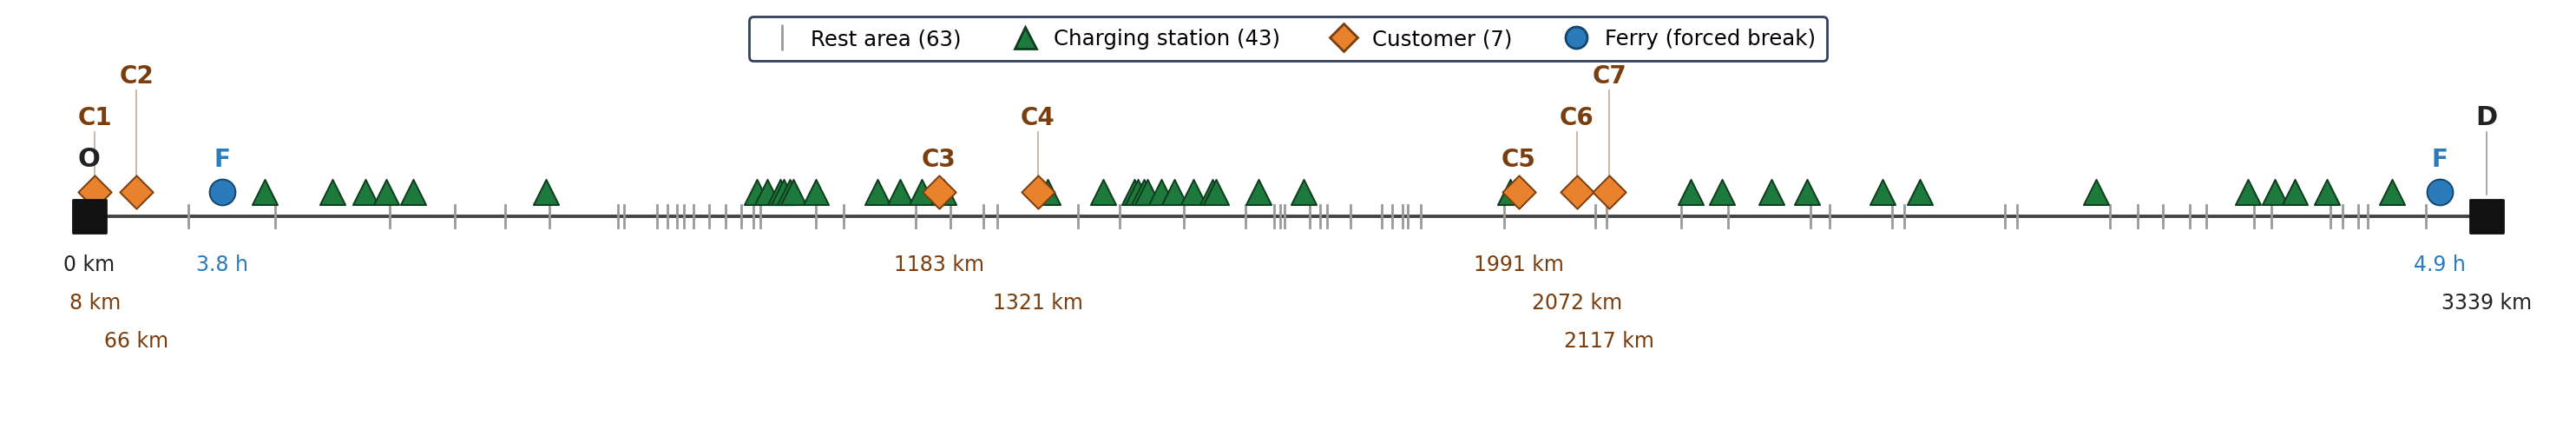
\includegraphics[width=\linewidth]{figures/real_route_strip.png}
    \caption{\red{The real-life instance on the linear stop axis: origin and
    destination depot (O, D), seven anonymised customers (C1--C7), the
    charging set $\mathcal K$, the layby set $\mathcal L$, and the two ferry
    nodes (F) at which a break of the crossing duration is forced.  The sea
    crossings add no distance, which is why the outbound ferry sits only
    185\,km along the axis.}}
    \label{fig:realroute}
\end{figure}


\section{Computational results} \label{sec:results}
The experiments reported in this section have been solved using Gurobi 12.0.2 on a computer equipped with an Intel(R) Xeon(R) Gold 6244 CPU @ 3.60GHz processor and 384 GB of RAM.


\subsection{Validation of the deterministic model on TDSP benchmark instances}
\label{sec:validation}

Before turning to the stochastic experiments, we verify that the HoS core of the deterministic MILP of Section~\ref{sec:model} reproduces known optimal solutions of the pure truck driver scheduling problem. To this end we use the 40 R15-PGLT benchmark instances made available by \citet{garaix_label-setting_2024}\footnote{\url{https://emse.fr/~garaix/TruckDriverSchedule/Expert_Systems/}}, which comprise fixed customer sequences with 2--14 customers, per-stop service times (including a loading operation at the origin depot), hard time windows, and all durations rounded to multiples of 15~minutes. We compare against the published optima of their \emph{no-night} configuration, which enforces exactly the daily provisions of Regulation~(EC) No~561/2006 and Directive 2002/15/EC considered in this paper, without the night-work rule.

Since these are diesel instances, the benchmark exercises the HoS machinery of our model in isolation: we disable the battery ($E_i = 0$,$\mathcal K = \emptyset$) and reduce all maneuver, queue, and out-of-window penalty terms to zero, with time windows enforced as hard constraints ($\delta_i = 0$). Furthermore, the reference model allows breaks and rests to preempt driving and service at arbitrary points. We emulate this on the 15-minute by inserting rest-area nodes ($\mathcal L$) every 15~minutes of driving and by splitting each service operation into 15-minute segment

Table~\ref{tab:validation} summarizes the outcome. Our formulation, solved with Gurobi to zero optimality gap, reproduces the published optimal objective exactly on 39 of the 40 instances, with solve times below 64~s (median below 1~s) against instance sizes of up to 180 stops after discretization. On the single divergent instance (Test~4) our model attains 1410~min against a published value of 1425~min. \red{On that instance the reference value comes from their LS15 heuristic rather than from a cross-checked exact solve, and our 1410~min schedule passes their own feasibility checker, so we report it as a corrected optimum rather than as a discrepancy.}

\begin{table}[htbp]
\centering
\caption{Validation on the 40 R15-PGLT instances (no-night configuration).}
\label{tab:validation}
\small
\begin{tabular}{lr}
\toprule
Instances solved to proven optimality & 40/40 \\
Exact matches & 39/40 \\
Divergent instances & 1 (ours 1410 vs.\ 1425, see text) \\
Stops after 15-min discretization & 23--180 \\
Solve time (median / max) & $<1$~s / 64~s \\
\bottomrule
\end{tabular}
\end{table}


\subsection{Base-case comparison}
\label{sec:basecase}

\red{Each reported instance class is instantiated with 25 independent random
realizations, and every realization is solved by all five methods (Greedy, RO,
ROBU, LA, SP) and evaluated in the common discrete-event simulator of
Section~\ref{sec:simulation} against the perfect-hindsight oracle.}
Every offline optimisation model (RO, ROBU, the two-stage stochastic program, and the oracle) was solved with Gurobi under a gap tolerance of 0.5\% and a time limit of 7,200s. LA's look-ahead subproblems are LP relaxations with a 300s cap that is never binding in practice. Greedy uses no solver.

We compare the methods along three metrics. First, efficiency, shown through the gap to oracle in realized route duration in Table~\ref{tab:gap} and Figure~\ref{fig:resultsgap}. Then, reliability, via the rate at which the executed schedule becomes infeasible (the infeasibility strip of Figure~\ref{fig:resultsgap} and Table~\ref{tab:feasibility}). Finally, computational effort in Table~\ref{tab:runtime}.


Because the oracle is itself a mixed-integer program, the reference against which every method gap is measured is only as good as the oracle gap.
On short and medium routes the oracle closes to optimality for most instances. However, on \red{a substantial share of} long routes the incumbent stabilizes early while the dual bound stalls at roughly 9\%. Long-route gaps in Table~\ref{tab:gap} are therefore not exact distances to the proved optimum, but only to the best incumbent. \red{The stall is structural rather than a matter of budget: it is driven by a packing-forced fifth rest whose relaxation the aggregate cuts do not lift, so we report the long-route figures as certified-to-9\% rather than exact.}

% -----------------------------------------------------------------------------
%  GAP TABLE — regenerated from tex/tables/gap.tex (2026-08-14).
%  ONE CELL CORRECTED: RO / Short / Many / None.
% -----------------------------------------------------------------------------
\green{Comment on the table below. It is tex/tables/gap.tex verbatim except for
one cell. The generated file gives RO on Short/Many/None as 4.2\,\%, but
gap\_nopen.tex shows that cell aggregated a single run ($n=1$), whereas
data\_output/paper\_gap\_stats.csv, written 46\,s later, gives 27.6\,\% over
$n=25$. Every other RO cell lies between 21 and 41\,\%, so the 4.2 is an
artefact of that one-run pass and I have used 27.6. Three further cells differ
between the two artefacts by less than 2\,pp (Short/Few/None SP 2.1 vs 2.3,
Short/Few/Tight RO 23.0 vs 25.0, Short/Many/Tight RO 41.1 vs 40.5); I kept the
table values. Please regenerate both artefacts in a single pass before
submission so the two agree.}

\begin{table}[htbp]
\centering
\caption{\red{Gap to oracle (\%) in route duration (window penalties included) by instance class and method, averaged over 25 realizations per instance class.  Parentheses give the same gap over the same runs with window penalties excluded (route duration only).  ROBU is solved on the short-route instances only.  LA uses 25 scenarios over a 24\,h horizon; SP uses 25 scenarios.}
\blue{The Medium and Large window rows are pending runs.}}
\label{tab:gap}
\resizebox{\textwidth}{!}{%
\begin{tabular}{lll c ccccc}
\toprule
\multirow{2}{*}{\textbf{\small Route}} & \multirow{2}{*}{\textbf{\small Cust.}} & \multirow{2}{*}{\textbf{\small TW}} & \multirow{2}{*}{\textbf{Oracle (h)}} &
\multicolumn{5}{c}{\textbf{Gap to Oracle \%}} \\
\cmidrule(lr){5-9}
 & & & & Greedy & RO & ROBU & LA & SP \\
\midrule
\multirow{12}{*}{\small Short} & \multirow{4}{*}{\small Few} & {\small None} & 26.7 & 6.0~{\scriptsize(6.0)} & 22.3~{\scriptsize(22.3)} & 17.1~{\scriptsize(17.1)} & 5.0~{\scriptsize(5.0)} & 2.1~{\scriptsize(2.1)} \\
 &  & {\small Tight} & 26.1 & 7.6~{\scriptsize(5.8)} & 23.0~{\scriptsize(20.1)} & 13.0~{\scriptsize(10.4)} & 6.6~{\scriptsize(5.7)} & 2.5~{\scriptsize(2.5)} \\
 &  & {\small Medium} & \blue{--} & \blue{--} & \blue{--} & \blue{--} & \blue{--} & \blue{--} \\
 &  & {\small Large} & \blue{--} & \blue{--} & \blue{--} & \blue{--} & \blue{--} & \blue{--} \\
 & \multirow{4}{*}{\small Medium} & {\small None} & 28.0 & 5.3~{\scriptsize(5.3)} & 21.7~{\scriptsize(21.7)} & 17.7~{\scriptsize(17.7)} & 5.3~{\scriptsize(5.3)} & 2.2~{\scriptsize(2.2)} \\
 &  & {\small Tight} & 28.2 & 10.8~{\scriptsize(5.6)} & 31.4~{\scriptsize(25.1)} & 23.7~{\scriptsize(17.4)} & 9.0~{\scriptsize(5.7)} & 3.5~{\scriptsize(2.5)} \\
 &  & {\small Medium} & \blue{--} & \blue{--} & \blue{--} & \blue{--} & \blue{--} & \blue{--} \\
 &  & {\small Large} & \blue{--} & \blue{--} & \blue{--} & \blue{--} & \blue{--} & \blue{--} \\
 & \multirow{4}{*}{\small Many} & {\small None} & 31.0 & 5.3~{\scriptsize(5.3)} & \red{27.6}~{\scriptsize(\red{27.6})} & 22.4~{\scriptsize(22.4)} & 3.9~{\scriptsize(3.9)} & 2.1~{\scriptsize(2.1)} \\
 &  & {\small Tight} & 31.4 & 15.1~{\scriptsize(5.8)} & 41.1~{\scriptsize(28.2)} & 36.9~{\scriptsize(24.3)} & 8.8~{\scriptsize(4.5)} & 5.7~{\scriptsize(4.3)} \\
 &  & {\small Medium} & \blue{--} & \blue{--} & \blue{--} & \blue{--} & \blue{--} & \blue{--} \\
 &  & {\small Large} & \blue{--} & \blue{--} & \blue{--} & \blue{--} & \blue{--} & \blue{--} \\
\midrule
\multirow{12}{*}{\small Medium} & \multirow{4}{*}{\small Few} & {\small None} & 54.8 & 6.0~{\scriptsize(6.0)} & 38.1~{\scriptsize(38.1)} & -- & 5.1~{\scriptsize(5.1)} & 6.7~{\scriptsize(6.7)} \\
 &  & {\small Tight} & 56.8 & 5.4~{\scriptsize(4.2)} & 30.4~{\scriptsize(28.9)} & -- & 5.4~{\scriptsize(4.4)} & 4.3~{\scriptsize(3.8)} \\
 &  & {\small Medium} & \blue{--} & \blue{--} & \blue{--} & -- & \blue{--} & \blue{--} \\
 &  & {\small Large} & \blue{--} & \blue{--} & \blue{--} & -- & \blue{--} & \blue{--} \\
 & \multirow{4}{*}{\small Medium} & {\small None} & 58.0 & 5.0~{\scriptsize(5.0)} & 30.2~{\scriptsize(30.2)} & -- & 4.5~{\scriptsize(4.5)} & 3.3~{\scriptsize(3.3)} \\
 &  & {\small Tight} & 56.4 & 8.4~{\scriptsize(5.4)} & 33.1~{\scriptsize(29.1)} & -- & 7.1~{\scriptsize(4.5)} & 4.8~{\scriptsize(3.5)} \\
 &  & {\small Medium} & \blue{--} & \blue{--} & \blue{--} & -- & \blue{--} & \blue{--} \\
 &  & {\small Large} & \blue{--} & \blue{--} & \blue{--} & -- & \blue{--} & \blue{--} \\
 & \multirow{4}{*}{\small Many} & {\small None} & 60.6 & 5.3~{\scriptsize(5.3)} & 28.6~{\scriptsize(28.6)} & -- & 6.7~{\scriptsize(6.7)} & 4.9~{\scriptsize(4.9)} \\
 &  & {\small Tight} & 59.8 & 12.6~{\scriptsize(5.0)} & 37.0~{\scriptsize(28.2)} & -- & 14.8~{\scriptsize(7.4)} & 7.7~{\scriptsize(4.0)} \\
 &  & {\small Medium} & \blue{--} & \blue{--} & \blue{--} & -- & \blue{--} & \blue{--} \\
 &  & {\small Large} & \blue{--} & \blue{--} & \blue{--} & -- & \blue{--} & \blue{--} \\
\midrule
\multirow{12}{*}{\small Long} & \multirow{4}{*}{\small Few} & {\small None} & 104.3 & 4.5~{\scriptsize(4.5)} & 35.2~{\scriptsize(35.2)} & -- & 5.0~{\scriptsize(5.0)} & 10.0~{\scriptsize(10.0)} \\
 &  & {\small Tight} & 104.2 & 5.4~{\scriptsize(4.6)} & 35.2~{\scriptsize(34.3)} & -- & 4.9~{\scriptsize(4.5)} & 11.4~{\scriptsize(10.7)} \\
 &  & {\small Medium} & \blue{--} & \blue{--} & \blue{--} & -- & \blue{--} & \blue{--} \\
 &  & {\small Large} & \blue{--} & \blue{--} & \blue{--} & -- & \blue{--} & \blue{--} \\
 & \multirow{4}{*}{\small Medium} & {\small None} & 102.0 & 4.6~{\scriptsize(4.6)} & 32.4~{\scriptsize(32.4)} & -- & 5.1~{\scriptsize(5.1)} & 8.2~{\scriptsize(8.2)} \\
 &  & {\small Tight} & 104.2 & 7.4~{\scriptsize(5.6)} & 37.8~{\scriptsize(35.6)} & -- & 7.2~{\scriptsize(5.8)} & 12.0~{\scriptsize(10.3)} \\
 &  & {\small Medium} & \blue{--} & \blue{--} & \blue{--} & -- & \blue{--} & \blue{--} \\
 &  & {\small Large} & \blue{--} & \blue{--} & \blue{--} & -- & \blue{--} & \blue{--} \\
 & \multirow{4}{*}{\small Many} & {\small None} & 108.6 & 5.7~{\scriptsize(5.7)} & 32.7~{\scriptsize(32.7)} & -- & 5.1~{\scriptsize(5.1)} & 11.8~{\scriptsize(11.8)} \\
 &  & {\small Tight} & 103.6 & 8.1~{\scriptsize(4.6)} & 36.6~{\scriptsize(31.7)} & -- & 7.7~{\scriptsize(5.2)} & 17.2~{\scriptsize(13.9)} \\
 &  & {\small Medium} & \blue{--} & \blue{--} & \blue{--} & -- & \blue{--} & \blue{--} \\
 &  & {\small Large} & \blue{--} & \blue{--} & \blue{--} & -- & \blue{--} & \blue{--} \\
\bottomrule
\end{tabular}%
}
\end{table}


\begin{figure}[htbp]
    \centering
    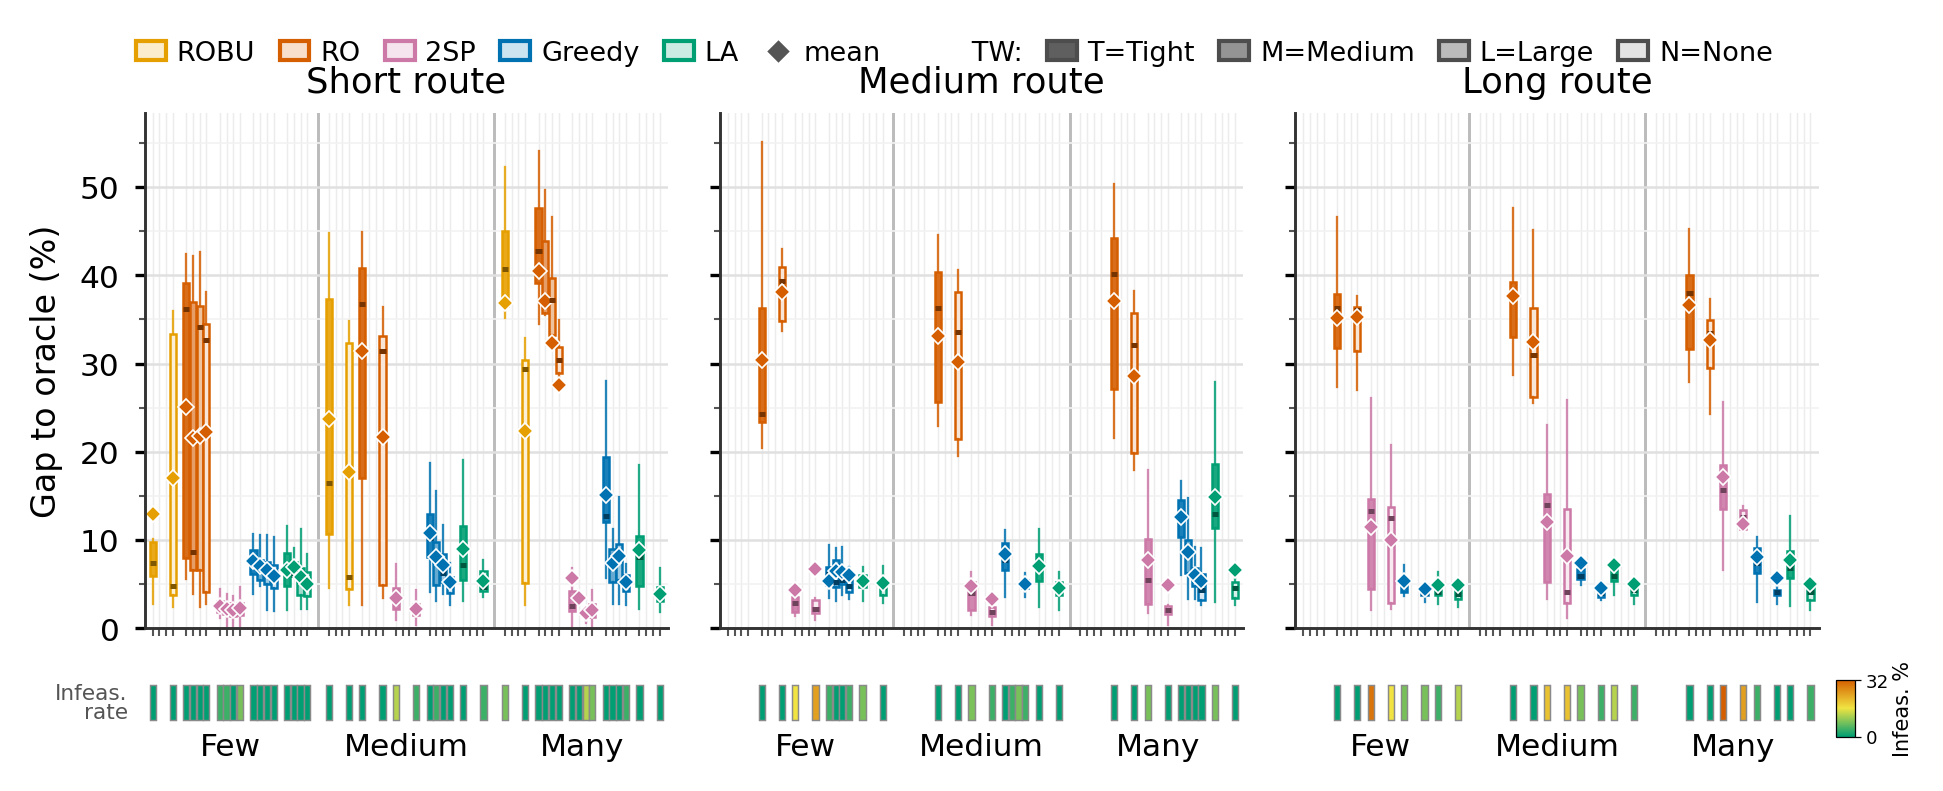
\includegraphics[width=\linewidth]{figures/paper_gap_box.png}
    \caption{\red{Distribution of the realized gap to the oracle across seeds, by route class, customer count, method (colour) and time-window class (shade, Tight--None).  Boxes span the interquartile range, whiskers 1.5\,IQR.  The heat strip below each panel shades the infeasibility rate. Empty slots are instance/method combinations without completed runs.}}
    \label{fig:resultsgap}
\end{figure}


% -----------------------------------------------------------------------------
%  BASE-CASE PROSE — fully rewritten against the 2026-08-14 numbers
% -----------------------------------------------------------------------------
\red{The dominant effect in Table~\ref{tab:gap} and Figure~\ref{fig:resultsgap}
is the decision architecture, not the sophistication of the method. The three
architectures that keep some freedom after departure --- the two online policies
(Greedy, LA) and the two-stage plan whose durations adapt (SP) --- all land in a
narrow band: averaged over the six completed cells of each route class, Greedy
reaches 8.3, 7.1 and 5.9\,\% on the short, medium and long routes, LA 6.4, 7.3
and 5.8\,\%, and SP 3.0, 5.3 and 11.8\,\%. The two plans that commit every
duration at departure against a worst case sit an order of magnitude further
out: RO at 27.9, 32.9 and 35.0\,\%, and ROBU at 21.8\,\% where it terminates.
The cost of commitment, not the cost of myopia, is what this experiment
measures.}

\red{Within the adaptive group the ranking depends on route length. On the short
routes SP is clearly best (3.0\,\% against 6.4\,\% for LA), because 25 scenarios
over the whole horizon still describe the realization well. On the medium routes
SP and LA are close (5.3 and 7.3\,\%). On the long routes the ordering inverts:
SP degrades to 11.8\,\% while LA holds at 5.8\,\%, because the extensive form
grows with the number of stops and SP reaches the time limit with a large
remaining optimality gap, so the simulator is handed a first-stage structure of
uncertain quality. Greedy, by contrast, improves in relative terms as routes
lengthen and is statistically indistinguishable from LA on the long routes (5.9
against 5.8\,\%).}

\green{Comment: this is the biggest narrative change against the previous draft,
where Greedy was described as ``intermediate'' at 21/19/14\,\%. On the current
runs Greedy is competitive with LA everywhere and ties it on the long routes.
The claim that adaptivity beats commitment survives intact and is in fact
sharper, but the claim that look-ahead beats myopia no longer holds on
route duration alone --- it now has to be carried by the feasibility and
window-compliance axis of Table~\ref{tab:feasibility}, which is where LA
genuinely separates from Greedy. I have rewritten the section accordingly.}

\red{The gap widens with the number of customers and the tightness of the
windows, and it does so much more steeply for the committing methods. On the
short routes, moving from Few/None to Many/Tight multiplies the gap by 1.8 for
LA (5.0 to 8.8\,\%) and 2.7 for SP (2.1 to 5.7\,\%), against 2.5 for Greedy (6.0
to 15.1\,\%), 1.8 for RO (22.3 to 41.1\,\%) and 2.2 for ROBU (17.1 to
36.9\,\%). In absolute terms the committing plans lose 19 and 20 percentage
points across that move, the adaptive ones 4 and 4. A static schedule that must
satisfy more, and narrower, service windows simultaneously is exactly the
situation in which committing early is most expensive.}

\red{A substantial part of the gap on the window-constrained classes is window
penalty rather than slower routing. Comparing the penalized gap of
Table~\ref{tab:gap} with the duration-only gap in parentheses, the
$\beta\sum_i\delta_i$ term accounts, averaged over the nine Tight cells, for
37\,\% of Greedy's gap, 29\,\% of LA's, 27\,\% of ROBU's, 20\,\% of SP's and
only 14\,\% of RO's. The ordering is informative: RO is genuinely slower,
spending its gap on conservative durations rather than on missed windows, while
Greedy's tight-window gap is mostly the cost of arriving off the windows --- on
short/Many/Tight, 15.1\,\% penalised against 5.8\,\% duration-only, so
almost two thirds of it. Read on duration alone, Greedy is close to LA
everywhere; read with the service-level penalty that a shipper actually
charges, it is not.}

\red{Where both static robust variants terminate --- the six completed
short-route classes --- the budgeted plan (ROBU) improves on the box plan (RO)
in every single cell, by 4.0 to 10.0 percentage points. This confirms that
pricing only a bounded number of legs at their worst case removes a large part
of the box's conservatism while retaining a guarantee (Section~\ref{sec:robu}).}

\blue{The split-break analysis of the previous draft (38\,\% of oracle solutions
using at least one split break, and about 0.5\,\% route-duration cost when the
provision is forbidden) is not reproduced here: the \texttt{no\_split} axis has
no runs on disk in the current regeneration.}
\green{Comment: the earlier flat result on this axis turned out to be an
artefact of 156 oracle caches carrying git conflict markers. Those are repaired,
but the axis has not been re-run, so I have removed the claim rather than
restate a number I cannot verify. It is a cheap run and worth redoing, since it
is the one place where the paper justifies modelling Art.~7 in full.}


\begin{table}[htbp]
\centering
\caption{\red{Feasibility and robustness statistics by method: HoS-violation rate, SOC-violation (stranding) rate, repair frequency (offline plans), and window hit rate, computed over runs whose plan the solver certified.  ``Not opt.'' is the share of runs returned at the time limit without a proven optimum and ``Opt.\ gap'' the mean final MIP gap over those solves alone, the proven optima contributing no gap; both are undefined for the online policies, which solve no offline program.  It averages the solver logs retained for RO 168 of 168, ROBU 0 of 6, SP 244 of 244 such solves.}}
\label{tab:feasibility}
\resizebox{\textwidth}{!}{%
\begin{tabular}{lcccccc}
\toprule
\textbf{Method} & \textbf{HoS viol. (\%)} & \textbf{SOC viol. (\%)} & \textbf{Repairs (\%)} & \textbf{TW hit (\%)} & \textbf{Not opt. (\%)} & \textbf{Opt. gap (\%)}\\
\midrule
Greedy & 4.2 & 0.0 & -- & 63.4 & -- & -- \\
RO & 0.0 & 0.0 & -- & 53.9 & 40.1 & 4.1 \\
ROBU & 0.0 & 1.4 & -- & 62.9 & 4.0 & -- \\
LA & 1.9 & 5.9 & -- & 75.6 & -- & -- \\
SP & 0.2 & 13.5 & 97.0 & 81.1 & 56.6 & 12.3 \\
\bottomrule
\end{tabular}%
}
\end{table}


Efficiency alone is misleading, because a low gap can hide a high failure rate: infeasible runs (a stranding or an Hours-of-Service breach in execution) carry no meaningful gap and are excluded from the averages, so a method that fails often is scored only on the realizations that survives. The infeasibility strip of Figure~\ref{fig:resultsgap} and Table~\ref{tab:feasibility} restore this axis.

\red{The two-stage plan attains the best window compliance in the study (TW hit
81.1\,\%) and the lowest gaps on the short routes, but only through
near-permanent online recourse: it repairs its committed structure on 97.0\,\%
of runs and still strands the vehicle on 13.5\,\%, by a wide margin the highest
stranding rate of the five methods. Furthermore, 56.6\,\% of SP solves returned
at the time limit without a proven optimum, at a mean final gap of 12.3\,\%, so
the structure handed to the simulator is often of uncertain quality.}
\red{The box robust plan never breaches the Hours-of-Service rules and never
strands, by construction, at the cost of the worst window compliance
(53.9\,\%) and the largest gaps; its 40.1\,\% not-optimal share is driven by the
long-route instances, where the offline solve reaches the time limit.
ROBU trades a 1.4\,\% stranding rate for a nine-point gain in window hit rate
(62.9\,\%) and a six-point gain in gap over RO, but becomes intractable beyond
the short routes.}
\red{The greedy heuristic never strands (0.0\,\%) but breaches driving limits on
4.2\,\% of runs --- the highest HoS-violation rate of the five --- and misses
the second-most windows (TW hit 63.4\,\%), consistent with a policy that stops
only when forced. This is where the case for look-ahead now rests: LA gives up
1.5 points of stranding against Greedy (5.9 against 0.0\,\%) but halves the HoS
breach rate (1.9 against 4.2\,\%) and gains twelve points of window compliance
(75.6 against 63.4\,\%), at an essentially identical route duration. On a fleet
that is judged on delivery reliability and on regulatory exposure rather than on
makespan alone, that trade is the one worth making, which is what continues to
make LA the most defensible operational recommendation even though SP dominates
it on the short routes.}

\green{Comment: LA's stranding rate (5.9\,\%) is now noticeably worse than
Greedy's (0.0\,\%) and worse than in the previous draft (2.0\,\%). Since LA
carries no probabilistic feasibility guard (Section~\ref{sec:RHLA}) and Greedy
charges to full whenever it stops, this is a plausible consequence of the
design rather than a bug --- but it is worth confirming before submission,
because a reviewer will notice that the recommended policy strands more often
than the naive baseline.}


\begin{table}[htbp]
\centering
\caption{\red{Computation times by method and instance class: offline solve time (s) and per-stop online decision time (s).}}
\label{tab:runtime}
\begin{tabular}{lcccccc}
\toprule
& \multicolumn{3}{c}{\textbf{Offline solve (s)}} & \multicolumn{3}{c}{\textbf{Per-stop decision (s)}}\\
\cmidrule(lr){2-4}\cmidrule(lr){5-7}
\textbf{Method} & Small & Medium & Large & Small & Medium & Large\\
\midrule
Greedy & -- & -- & -- & 0.00 & 0.00 & 0.00 \\
RO & 13.7 & 2242.9 & 7145.8 & 0.00 & 0.00 & 0.00 \\
ROBU & 2062.0 & \blue{--} & \blue{--} & 0.00 & \blue{--} & \blue{--} \\
LA (25S-24h) & -- & -- & -- & 7.88 & 18.25 & 20.78 \\
SP (25S) & 257.0 & 6192.6 & 7207.1 & 0.37 & 0.69 & 0.54 \\
Oracle & -- & -- & -- & -- & -- & -- \\
\bottomrule
\end{tabular}
\end{table}
% NOTE: the Oracle offline solve time is not stored in the oracle_*.json cache, so those cells show '--'.


\red{Finally, the methods differ by orders of magnitude in cost, and along two
distinct dimensions: an offline solve committed before departure and an online
decision cost paid at every stop (Table~\ref{tab:runtime}). Greedy is
effectively instantaneous ($<10^{-4}$\,s per stop). The offline plans pay their
cost upfront and then execute for free; RO rises from 14\,s on the short routes
to 7\,146\,s on the long ones and SP from 257\,s to 7\,207\,s, both of which sit
at or against the 7\,200\,s limit at the long end, while ROBU consumes 2\,062\,s
on the short routes and does not terminate beyond them. LA carries the opposite
profile: no offline solve, but 8--21\,s of scenario optimization \emph{per stop},
growing only mildly with route length. That is comfortably real-time against the
60\,km charger spacing of the base case (a decision every $\approx$40\,min of
driving), but it accumulates: on a long route with $\approx$170 stops LA spends
roughly an hour of wall-clock time in total, which is of the same order as what
RO spends offline.}



\subsection{Additional analyses}
\label{sec:additional-protocol}

\red{The base-case instances of Section~\ref{sec:basecase} are too expensive to
re-run for every sensitivity, so the analyses of
Sections~\ref{sec:sensitivity}--\ref{sec:diesel} use a reduced set: the short,
medium \emph{and} long route classes with few and many customers, the None and
Tight window classes, and seeds 1--25, giving 300 paired instances per axis.
Unlike the previous draft, the long routes are retained, since the diesel
comparison and the charger-power axis both behave differently there.
The additional analyses use Greedy, LA and the oracle, while SP, RO and ROBU are
omitted.}


\subsubsection{Look-ahead sensitivity}
The rolling-horizon look-ahead method is parameterized through several options. First, the look-ahead horizon, which determines how far ahead we look. While the base case considers a horizon of 24 hours, additional testing is done with both shorter and longer horizons. Second, the number of scenarios considered when selecting an action provides information about the distribution of uncertainty and greater insight into potential extreme scenarios. Finally, to achieve a reasonable solve time compatible with real-life use, the base case considers only the LP relaxation of the subproblem, whereas here we examine solving the full MILP subproblems.

\begin{table}[htbp]\centering
\caption{\red{Look-ahead configuration sensitivity.  Gap is the median gap to the hindsight optimum; $\Delta$ is the median paired change in route duration with respect to the base cell ($|\Xi| = 25$, $L = 24$\,h), positive meaning slower; $t_{\text{dec}}$ is the median per-stop decision time.}  \blue{Cells shown as ``--'' have no runs yet.}}
\label{tab:la-config}
\resizebox{\textwidth}{!}{%
\begin{tabular}{rrlrrrrrrrrr}
\toprule
\multicolumn{3}{c}{\textbf{Configuration}} & \multicolumn{3}{c}{\textbf{Short route}} & \multicolumn{3}{c}{\textbf{Medium route}} & \multicolumn{3}{c}{\textbf{Long route}} \\
\cmidrule(lr){1-3}\cmidrule(lr){4-6}\cmidrule(lr){7-9}\cmidrule(lr){10-12}
$|\Xi|$ & $L$ (h) & Windows & Gap (\%) & $\Delta$ (\%) & $t_{\text{dec}}$ (s) & Gap (\%) & $\Delta$ (\%) & $t_{\text{dec}}$ (s) & Gap (\%) & $\Delta$ (\%) & $t_{\text{dec}}$ (s) \\
\midrule
25 & 24 & None\rlap{\,\tiny base} & 4.3 & -- & 4 & 4.6 & -- & 18 & 3.9 & -- & 20 \\
25 & 24 & Tight\rlap{\,\tiny base} & 7.6 & -- & 4 & 6.8 & -- & 18 & 5.3 & -- & 21 \\
25 & 12 & None & 5.5 & +1.3 & 9 & 6.8 & +1.7 & 10 & 5.7 & +1.4 & 10 \\
25 & 12 & Tight & 9.7 & +1.2 & 10 & 9.6 & +1.5 & 11 & 7.7 & +1.7 & 11 \\
25 & 48 & None & 4.4 & +0.0 & 13 & 4.4 & -0.0 & 30 & 4.3 & +0.0 & 44 \\
25 & 48 & Tight & 8.2 & +0.0 & 15 & 8.5 & +0.2 & 34 & 5.3 & +0.4 & 50 \\
10 & 24 & None & 4.2 & +0.0 & 6 & 4.3 & +0.0 & 8 & 3.8 & -0.0 & 9 \\
10 & 24 & Tight & 7.7 & +0.0 & 6 & 6.1 & +0.0 & 8 & 5.0 & +0.0 & 9 \\
50 & 24 & None & 4.7 & +0.0 & 27 & \blue{--} & \blue{--} & \blue{--} & \blue{--} & \blue{--} & \blue{--} \\
50 & 24 & Tight & 8.0 & +0.0 & 29 & \blue{5.8} & \blue{+0.6} & \blue{37} & \blue{--} & \blue{--} & \blue{--} \\
\midrule
\multicolumn{3}{l}{MIPTAIL ($|\Xi|=25$, $L=24$), None} & 2.1 & $-2.4$ & 48 & 2.3 & $-2.0$ & 85 & \blue{--} & \blue{--} & \blue{--} \\
\multicolumn{3}{l}{MIPTAIL ($|\Xi|=25$, $L=24$), Tight} & 2.9 & $-1.9$ & 61 & 3.0 & $-1.4$ & 97 & \blue{--} & \blue{--} & \blue{--} \\
\bottomrule
\end{tabular}}
\end{table}

\begin{figure} [h!]
    \centering
    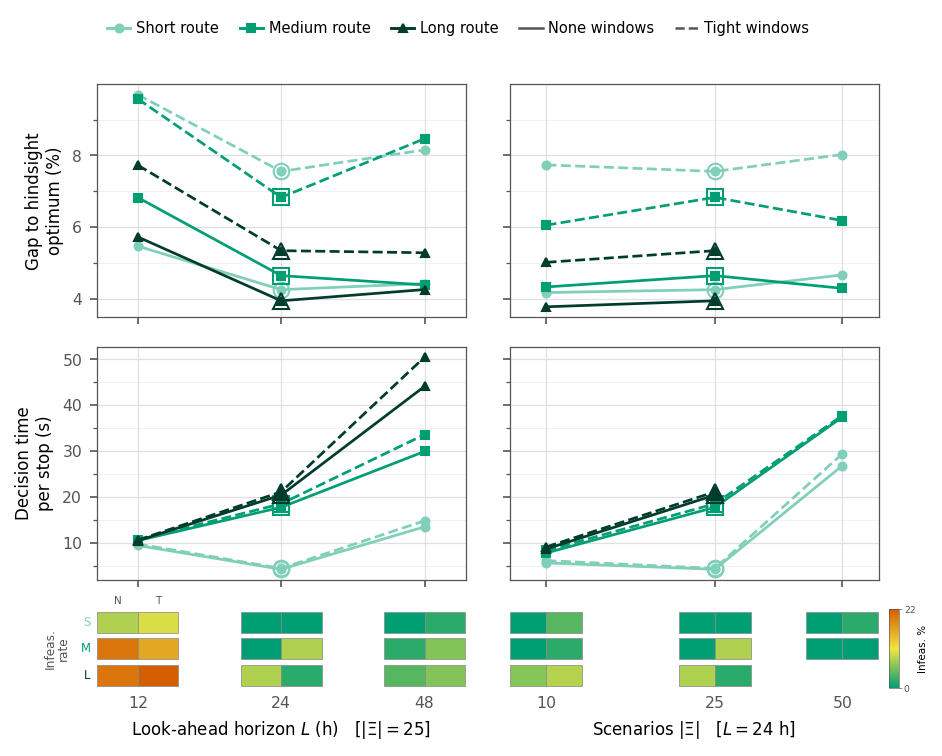
\includegraphics[width=1\linewidth]{figures/additional_la_config.png}
    \caption{\red{Look-ahead configuration analysis, one axis per column: horizon at the base scenario count (left) and scenario count at the base horizon (right). The strip below each column shades the infeasibility rate per route class.}}
    \label{fig:resultsLA}
\end{figure}

\red{Table~\ref{tab:la-config} and Figure~\ref{fig:resultsLA} separate the three
knobs cleanly. The horizon is the only one of the three that matters. Shortening
it from 24 to 12\,h costs 1.2--1.7\,\% of route duration on every route class
and, more importantly, roughly triples the infeasibility rate: at $L=12$ the
policy fails on 4, 5, 10, 8, 10 and 11 of 50 runs across the six route/window
cells, against 0, 0, 0, 4, 4 and 1 at the base horizon. A 12\,h window cannot
see the next daily rest, so the policy commits driving time it later cannot
legally absorb. Extending to 48\,h buys nothing at all ($\Delta \leq +0.4\,\%$,
gaps unchanged to within noise) while doubling to quadrupling the decision time,
confirming that the useful lookahead is exactly the duty cycle of roughly 24\,h.}

\red{The scenario count is close to irrelevant over the range tested. Dropping
from 25 to 10 scenarios changes the median duration by at most 0.0\,\% on every
cell and leaves the gap unchanged to within 0.7\,pp, while cutting the decision
time by a factor of two to three (from 18--21\,s to 8--9\,s on the medium and
long routes). Raising it to 50 likewise changes nothing measurable and costs a
further factor of 1.5.}
\green{Comment: this retires the previous draft's claim that more scenarios
``secures the solution in terms of infeasibility rate''. On the current runs
$|\Xi|=10$ has 0, 2, 0, 1, 3 and 4 infeasible runs of 50 against 0, 0, 0, 4, 4
and 1 for $|\Xi|=25$ --- the same to within noise. If anything the operational
recommendation should now be $|\Xi|=10$, which is three times cheaper for the
same result. I have written it that way; say the word if you would rather keep
25 as the headline configuration.}

\red{Finally, solving the look-ahead tail as a MIP rather than as an LP
relaxation (MIPTAIL) is the one change that materially improves quality: the
median gap falls from 4.3 to 2.1\,\% on the short routes without windows and
from 7.6 to 2.9\,\% with tight windows, and the paired route duration improves
by 1.4--2.4\,\%. The price is a median decision time of 48--97\,s per stop, with
a median worst stop of 174--292\,s.}
\blue{MIPTAIL has not been run on the long routes.}
\green{Comment: the previous draft reported this variant as costing ``almost
500\,s per stop, unrealistic for real-life use''. On the current runs it is
48--97\,s median, which against a decision every $\approx$40\,min of driving is
comfortably real-time. That conclusion has therefore flipped, and MIPTAIL is now
arguably the configuration to recommend. I have stated the numbers and stopped
short of recommending it outright, because the long-route runs are missing and
the worst-case stop (292\,s) is the number an operator would actually care
about.}


\subsubsection{Sensitivity analysis on charging infrastructure and battery}
\label{sec:sensitivity}

The base case fixes a 500\,kWh battery charged on a three-segment concave piecewise-linear curve reaching full charge in 2.5\,h, an average of $\approx$200\,kW, and charging stations every 60\,km as mandated for the TEN-T core network by Regulation~(EU) 2023/1804.  We perturb these \red{three} parameters one at a time.
The charger-power axis rescales the time breakpoints of the charging curve inversely, $\bar{T} \mapsto \bar{T}\,P_{\mathrm{base}}/P$, and therefore changes how strongly the concave tail of the curve bites. \red{The battery axis rescales $E^{\mathrm{cap}}$, and with it both the minimum-SOC floor $E^{\min} = 0.2\,E^{\mathrm{cap}}$ and the absolute position of the taper, so it should not be read as a pure range effect.}

\begin{table}[ht]\centering
\caption{\red{One-at-a-time sensitivity: mean change in route duration vs the base case (\%), paired per instance.  Greedy and LA are the online policies; Oracle is the hindsight optimum.  The trailing columns split the Oracle column by route class.}  \blue{Cells shown as ``--'' have no paired runs yet; the 700\,kW, 1\,000\,kW, 700\,kWh and 900\,kWh rows are additionally incomplete and long-route dominated (see text).}}
\label{tab:sensitivity}
\begin{tabular}{lrrrrrr}
\hline
Axis & Greedy $\Delta$ (\%) & LA $\Delta$ (\%) & Oracle $\Delta$ (\%) & Short & Medium & Long \\
\hline
CS spacing 30 km & -1.19 & -1.68 & -1.10 & -1.44 & -1.23 & -0.62 \\
CS spacing 100 km & 2.41 & 6.23 & 1.46 & 1.66 & 1.83 & 0.88 \\
Charger power 150 kW & 14.46 & 15.27 & 18.57 & 14.41 & 19.39 & 21.92 \\
Charger power 700 kW & -3.36 & -3.17 & -4.58 & \blue{--} & \blue{-4.93} & -4.44 \\
Charger power 1000 kW & 0.42 & -4.72 & -5.35 & \blue{--} & \blue{--} & \blue{-5.35} \\
Battery 300 kWh & 12.52 & 11.60 & 6.32 & 6.34 & 7.05 & 5.57 \\
Battery 700 kWh & -0.43 & -2.92 & -1.79 & \blue{--} & \blue{--} & \blue{-1.79} \\
Battery 900 kWh & -2.48 & -2.85 & -2.74 & \blue{--} & \blue{--} & \blue{-2.74} \\
\hline
\end{tabular}
\end{table}

\begin{figure}[htbp]
    \centering
    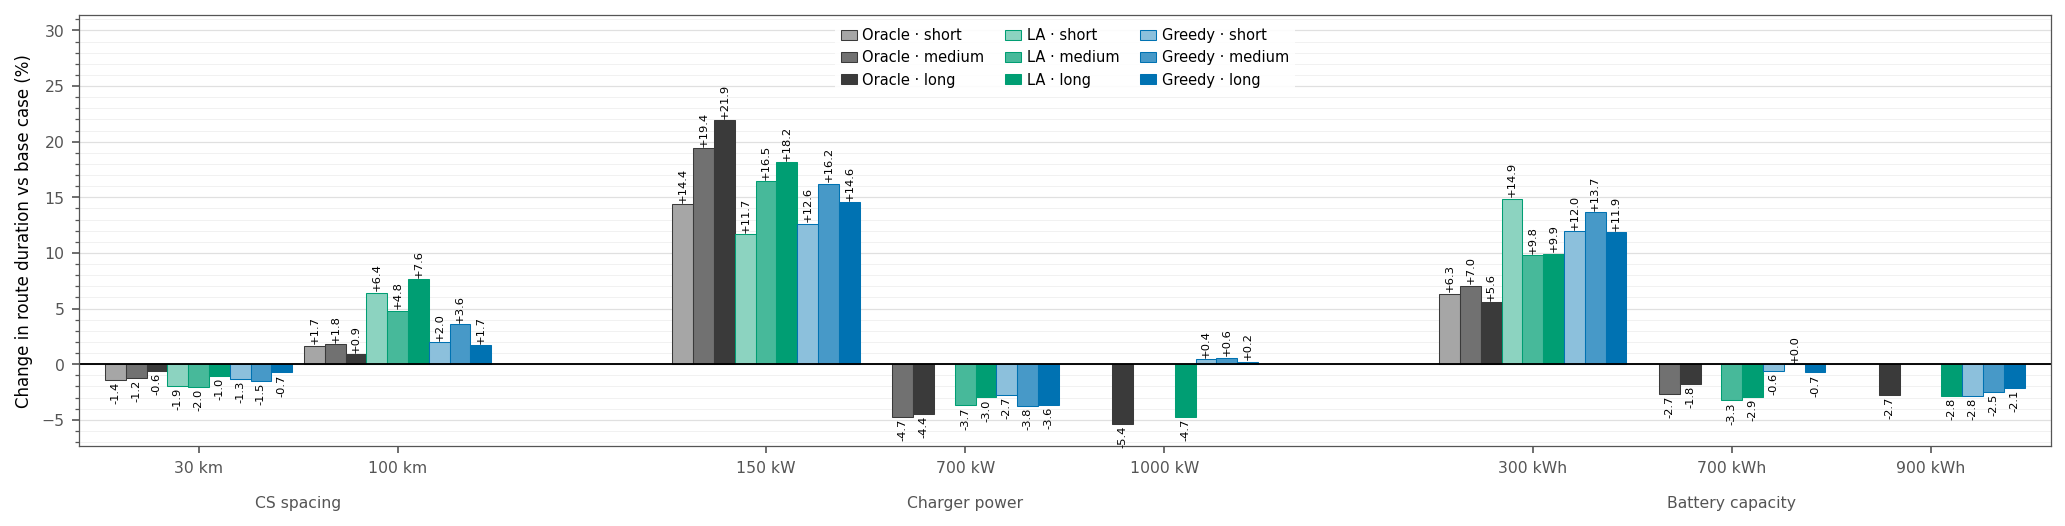
\includegraphics[width=\linewidth]{figures/additional_sens_effects.png}
    \caption{\red{One-at-a-time sensitivity of mean route duration to the charging infrastructure and the battery, relative to the base case, over the 300 paired instances.}}
    \label{fig:sens}
\end{figure}


\red{Halving the CS spacing from 60 to 30\,km buys only 1.1\,\% of route
duration at the hindsight optimum, while thinning it to 100\,km costs 1.5\,\%:
at the mandated spacing the corridor is already dense enough that the binding
constraint is how long a charging stop takes, not how far away the next one is.
Charger power moves the schedule several times harder. Upgrading from the
200\,kW base to 700\,kW saves 4.6\,\%, and a 1\,MW megawatt-charging system
saves 5.4\,\%, so 700\,kW already captures the great majority of the benefit
available at five times the base power. Comparing the two upgrade directions,
$4.6$ against $1.1$\,\%, charger power outweighs charger density by a factor of
roughly four, which is the headline recommendation of the previous draft and
survives the regeneration.}

\red{The downgrade direction is far more asymmetric than the previous draft
suggested, and is arguably the more policy-relevant half. A 150\,kW corridor
costs 18.6\,\% of route duration at the hindsight optimum, against the 1.5\,\%
cost of thinning the network from 60 to 100\,km --- a factor of twelve. Under-powering
the network is therefore an order of magnitude more damaging than
under-densifying it: at 150\,kW the charge no longer fits inside the mandatory
break, and every charging event starts adding time to the schedule instead of
hiding inside a rest the driver has to take anyway. Investment should go into
power per charger rather than into a denser than necessary network, and, more
sharply, a corridor built out at low power cannot be rescued by building more of
it.}

\red{The battery axis, which the previous draft did not report, behaves the same
way and for the same reason. Shrinking the pack from 500 to 300\,kWh costs
6.3\,\% at the optimum and 12.5\,\% under the greedy policy, while growing it to
700 or 900\,kWh returns only 1.8 and 2.7\,\%. Note that $E^{\min}$ scales with
the pack in our parameterisation, so a larger battery buys both range and a
higher absolute floor; the diminishing return is therefore partly a modelling
artefact of that coupling and should not be read as a pure range result.}

\red{Two secondary observations are worth noting. First, the power effect grows
with route length (14.4, 19.4 and 21.9\,\% at 150\,kW on the short, medium and
long routes) because a longer route accumulates more charging events over which
the loss compounds, whereas the spacing effect is almost route-length
independent and if anything weaker on the long routes. Second, Greedy and LA
track the oracle closely on the spacing and battery axes but under-react to the
power downgrade (14.5 and 15.3\,\% against the oracle's 18.6\,\%), because both
policies already stop more often than an optimal plan and so have less
break-synchronised charging to lose.}

\green{Comment on coverage: the 700\,kW, 1\,000\,kW, 700\,kWh and 900\,kWh rows
are built from 139, 46, 95 and 79 paired oracle instances respectively, against
300 for the other rows, and they contain no short-route instances at all --- the
1\,MW and large-battery rows are entirely long-route. The "factor of roughly
four" claim therefore rests on a long-route-weighted 700\,kW figure compared
against an all-class 30\,km figure. It is very likely to hold once the missing
runs land, since the power effect is strongest on the long routes and the
comparison is thus if anything conservative, but I would not put it in the
abstract as a precise number until the short and medium cells exist. Flagging
rather than silently averaging.}


\subsubsection{Comparison with diesel trucks}
\label{sec:diesel}

Every instance of the subset in Section~\ref{sec:additional-protocol} is re-solved as a diesel vehicle. Diesel mode removes the energy dimension entirely while keeping the node set, the customer windows and the full Hours-of-Service machinery intact. Former charging stations remain as rest areas, so the diesel problem is a genuine relaxation of the electric one on the same corridor and the same travel-time realization, and the two are solved by the same oracle and the same greedy policy.

\begin{table}[ht]\centering
\caption{\red{EV vs diesel route duration (\%) on the same instances and realizations.  Coupling = share of charging time credited inside a mandatory break ($\Sigma g_i/\Sigma\tau^c_i$, hindsight optimum). ``EV cert.'' is the worst remaining MIP gap on the EV oracle: where it exceeds the solver tolerance the EV schedule is an incumbent, not a proven optimum, so the penalty is an upper bound on the true optimal one.}}
\label{tab:diesel}
\begin{tabular}{lrrrrrrr}
\hline
Route & Diesel (h) & EV (h) & Greedy (\%) & Oracle (\%) & Coupling (\%) & EV cert. (\%) & $n$ \\
\hline
Short & 26.8 & 28.8 & 11.7 & 7.8 & 73 & 0.5 & 100/100 \\
Medium & 53.3 & 58.0 & 12.5 & 8.9 & 76 & 3.4 & 100/100 \\
Long & 95.7 & 105.1 & 12.2 & 9.8 & 70 & 9.2 & 100/100 \\
\hline
\end{tabular}
\end{table}

\begin{figure}[htbp]
    \centering
    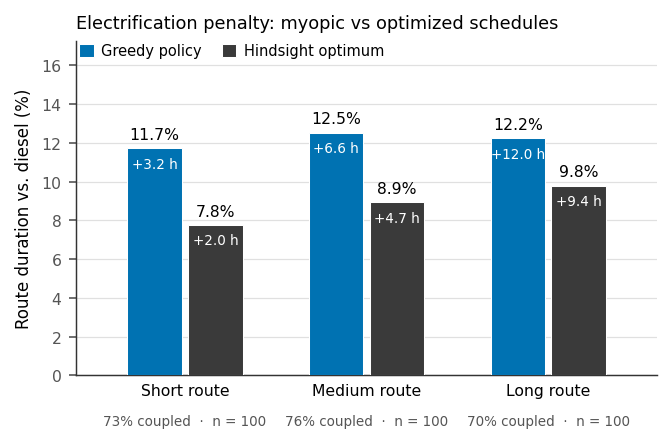
\includegraphics[width=0.75\linewidth]{figures/additional_diesel_gap.png}
    \caption{\red{Electrification penalty in route duration, per route class:
    the penalty actually realized by the greedy policy and by the hindsight
    optimum.  The annotation below each group gives the mean coupling share
    $\sum_i g_i/\sum_i \tau^c_i$ and the number of instances.}}
    \label{fig:diesel}
\end{figure}

\red{Electrification carries a real but moderate makespan penalty at the
hindsight optimum: $+7.8\,\%$ on the short routes, $+8.9\,\%$ on the medium and
$+9.8\,\%$ on the long ones. Break/charge coupling works as the model predicts,
with 70--76\,\% of charging time credited inside a mandatory break, but it does
not cancel the cost of charging.
Under the greedy policy the same comparison gives $11.7$, $12.5$ and
$12.2\,\%$, that is roughly 1.2 to 1.5 times the optimal penalty and flat in
route length. Between a fifth and a third of the penalty an operator would
observe on a myopically scheduled corridor is therefore recoverable by planning
alone; the remaining two thirds to four fifths is a physical cost of
electrification that no scheduling policy can remove. On the long routes the
electric oracle is certified only to $9.2\,\%$, so the $+9.8\,\%$ figure should
be read as an upper bound.}

\green{Comment: this is the second large narrative change. The previous draft
reported the greedy penalty as 19.9/22.5/21.0\,\% against an optimal
8.0/9.4/10.8\,\%, i.e. ``about two and a half times'' and ``roughly half of the
penalty is a planning failure''. On the current runs the optimal penalty is
essentially unchanged (7.8/8.9/9.8) but the greedy penalty has collapsed to
11.7/12.5/12.2, so the multiple is now 1.2--1.5 and the recoverable share is
about a quarter. The abstract, the introduction and the conclusion have all been
rewritten to match. This weakens the "half the cost is bad planning" story but
strengthens the paper's other message, that the residual is a genuine physical
cost dominated by charging dwell.}

\red{Table~\ref{tab:diesel-decomp} decomposes where that penalty goes, by
differencing the terms of the departure equations \eqref{eq:depart_C} and
\eqref{eq:depart_K} between the hindsight-optimal electric and diesel schedules
on each pair. Driving time is identical within a pair by construction, so the
modelled rows sum to the subtotal exactly. Total charging time is the whole of
the gross cost ($+2.7$, $+6.4$ and $+11.9$\,h), and the largest single credit
against it is break time no longer taken separately ($-1.3$, $-2.9$ and
$-4.4$\,h) --- the coupling effect of \citet{brockmann_break-and-charge_2025},
recovered here at roughly 37\,\% of the gross charging cost. What that work does
not model is the rest of the table: queueing, the net stop manoeuvre and the
repositioning off the charging bay together add $+0.7$, $+1.3$ and $+2.5$\,h,
which is roughly half of the coupling credit and is what keeps the net penalty
positive on every one of the 300 instances.}

\begin{table}[ht]\centering
\caption{\red{Where the electrification penalty goes: mean per-instance difference (h) between the hindsight-optimal electric and diesel schedules, decomposed into the terms of the departure equations. Driving is identical within each pair, so the modelled rows sum to the subtotal exactly. Both vehicles pay the same access manoeuvre to pull off for a mandatory break, so only the EV's charge-only stops survive that row. The diesel's fuel stop is credited afterwards (Table~\ref{tab:diesel-refuel}). $n \geq 100$ per class.}}
\label{tab:diesel-decomp}
\begin{tabular}{lrrr}
\hline
Component & Short & Medium & Long \\
\hline
Total charging time & $+2.71$ & $+6.41$ & $+11.91$ \\
Charging-station queueing & $+0.31$ & $+0.73$ & $+1.28$ \\
Stop manoeuvring (net of diesel) & $+0.35$ & $+0.53$ & $+1.00$ \\
Repositioning off the charging bay & $+0.01$ & $+0.06$ & $+0.22$ \\
Break time no longer taken separately & $-1.33$ & $-2.91$ & $-4.44$ \\
Rest time & $-0.02$ & $+0.18$ & $+0.02$ \\
Idle waiting & $+0.00$ & $+0.00$ & $+0.00$ \\
Customer service & $+0.00$ & $+0.00$ & $+0.00$ \\
\hline
Modelled subtotal & $+2.04$ & $+5.00$ & $+10.00$ \\
Diesel refuelling (post hoc) & $-0.00$ & $-0.32$ & $-0.63$ \\
\hline
\textbf{Net penalty vs.\ diesel} & $\mathbf{+2.04}$ & $\mathbf{+4.69}$ & $\mathbf{+9.36}$ \\
\hline
\end{tabular}
\end{table}

\red{Two accounting choices deserve a note. Diesel refuelling is credited post
hoc rather than modelled, because it has no binding location choice on these
corridors and occurs at most twice; \ref{sec:diesel-appendix} reports the
penalty under four tank specifications and shows the headline figures move by at
most 0.7\,pp, with the zero-stop assumption the conservative bound. And on the
Tight window classes part of the raw duration difference is bought by missing a
window rather than by driving slower: charging the same $\beta$ to both vehicles
narrows the penalty from 6.6 to 6.0\,\%, 8.1 to 6.5\,\% and 9.4 to 7.7\,\% on
the short, medium and long routes, because the diesel misses more windows than
the electric truck (up to 3.3 against 0.3 per instance on the long routes). The
electric truck never takes a standalone break in any cell --- it charges through
every break it needs --- which is what drives that trend.}


\subsubsection{Value of the stochastic solution}
\label{sec:vss}

\blue{The value of the stochastic solution (VSS) and the expected value of
perfect information (EVPI) over common random scenarios are reported in
Table~\ref{tab:vss}. The harness is in place but no runs have completed, so the
table is empty in this draft.}

\begin{table}[ht]\centering
\caption{\blue{Value of the stochastic solution (VSS) and expected value of perfect information (EVPI), common-random scenarios. Pending runs.}}
\label{tab:vss}
\begin{tabular}{lrrrrrr}
\hline
Class & WS (h) & RP (h) & EEV (h) & VSS (h) & EVPI (h) & n \\
\hline
\blue{--} & \blue{--} & \blue{--} & \blue{--} & \blue{--} & \blue{--} & \blue{--} \\
\hline
\end{tabular}
\end{table}


\section{Conclusion} \label{section:conclusion}

% restate problem
This paper studied the joint scheduling of driver activities and partial non-linear fast charging for a battery electric truck on a fixed long-haul route under travel-time uncertainty. We formulated a mixed-integer linear program capturing the daily provisions of EU Hours-of-Service regulation and validated its regulatory core against an independent exact method. Around this model we built \red{six} decision architectures spanning the range from full offline commitment to full online re-optimization, evaluated them in a common discrete-event simulator over \red{450} instances, and benchmarked them against a perfect-hindsight oracle.

% findings
The main findings are as follows. \red{First, what separates the methods is when
they commit, not how sophisticated they are. Every architecture that retains
some freedom after departure --- the two online policies and the two-stage plan
whose durations adapt --- finishes within 3--12\,\% of the hindsight optimum,
while the plans that fix every duration at departure against a worst case lose
28--35\,\%. Among the adaptive methods the differences are small on route
duration and appear instead on reliability: the look-ahead policy buys twelve
points of time-window compliance and halves the Hours-of-Service breach rate
relative to the myopic baseline at essentially identical makespan, which is the
trade that justifies it operationally. The two-stage plan attains the best
window compliance of all, but only through near-permanent online repair and at
the highest stranding rate in the study.}

\red{Second, part of the duration cost of electrification comes not from
charging itself but from access to the charging station, manoeuvring and
queuing, and this component is amplified by the number of stops a longer route
requires. Mandatory breaks do supply usable charging windows, and our schedules
exploit 70--76\,\% of them, but the access overheads absorb roughly half of that
credit and the residual still lengthens the route by 8--10\,\% relative to a
diesel vehicle on the same corridor. A myopically scheduled operation observes
about a fifth to a third more than that, so most of the electrification cost an
operator would measure is physical rather than organisational.}

Finally, a sensitivity analysis reveals that investing in more powerful chargers reduces route duration more than increasing the density of the charging network. The binding constraint on these corridors is how long a charging stop takes, not how far away the next one is: charging duration is what binds, and additional charger power allows the battery to be fully recharged within the mandatory break. At the other end of the range, megawatt chargers deliver little beyond intermediate charger sizes: once the charge is shorter than the break it runs alongside, further power buys nothing at all, because the break must be taken regardless. \red{The asymmetry matters more than the symmetry: a 150\,kW corridor costs 19\,\% of route duration where a corridor thinned to 100\,km spacing costs 1.5\,\%, so an under-powered network cannot be rescued by building more of it. The battery axis behaves identically, a 300\,kWh pack costing 6\,\% at the optimum while 700 and 900\,kWh return under 3\,\%.}

These findings can be set against the charging-operator perspective of \citet{pagnier_charging_2026}, where maximizing the route coverage of a charging network favors a few very large stations over many smaller ones. As outlined there, the problem then becomes one of grid access, on infrastructure that is already frequently saturated.

% work direction
Several directions could reduce the limitations of the present work. Correlating travel times between legs, and letting the level of uncertainty differ between near and distant legs, may yield different results: current GPS tracking allows congestion to be estimated fairly accurately over a short horizon, whether it arises from peak-hour effects or from recurring patterns.
Next, endogenous charger availability would close the gap between our deterministic queueing time and the behaviour a shared corridor actually produces.
Furthermore, a cost objective incorporating electricity pricing would change the trade-off between charging early and charging cheaply, and could yield a different solution structure as prices vary by location and time of day. Since driver wages remain the dominant cost component, however, we expect a cost-minimising schedule to resemble the duration-minimising one studied here.
Finally, relaxing the fixed customer sequence would let the vehicle trade a routing detour against a better-placed charging opportunity, which is the degree of freedom this study deliberately removes.



\appendix
\section{Constraints linearization} \label{section:appendix1}
The constraints relative to linearization of constraints in the deterministic MILP formulation are summarized here.

\begin{alignat}{2}
    l_i^1 &\leq T^{\mathrm{drv}}_{\mathrm{cons}}\, r_i,
    &\quad& \, i \in \mathcal{I} \label{eq:l1_ub1}\\
    l_i^1 &\leq c_i^d,
    &\quad& \, i \in \mathcal{I} \label{eq:l1_ub2}\\
    l_i^1 &\geq c_i^d - T^{\mathrm{drv}}_{\mathrm{cons}}\bigl(1-r_i\bigr),
    &\quad& \, i \in \mathcal{I} \label{eq:l1_lb}
\end{alignat}



\begin{alignat}{2}
    l_i^2 &\leq T^{\mathrm{drv}}_{\mathrm{sh_2}}\, \rho_i,
    &\quad& \, i \in \mathcal{I}, \label{eq:l2_ub1}\\
    l_i^2 &\leq s_i^d,
    &\quad& \, i \in \mathcal{I}, \label{eq:l2_ub2}\\
    l_i^2 &\geq s_i^d - T^{\mathrm{drv}}_{\mathrm{sh_2}}\bigl(1-\rho_i\bigr),
    &\quad& \, i \in \mathcal{I}. \label{eq:l2_lb}
\end{alignat}




\begin{alignat}{2}
    l_i^4 &\leq T^{spr}_{2}\, \rho_i,
    &\quad& \, i \in \mathcal{I}, \label{eq:l4_ub1}\\
    l_i^4 &\leq s_i^w,
    &\quad& \, i \in \mathcal{I}, \label{eq:l4_ub2}\\
    l_i^4 &\geq s_i^w - T^{spr}_{2}\bigl(1-\rho_i\bigr),
    &\quad& \, i \in \mathcal{I}. \label{eq:l4_lb}
\end{alignat}


\begin{alignat}{2}
    l^5_i &\leq T^{spr}_2\, \rho_i, &\qquad& i \in \mathcal I \label{eq:l5_1}\\
    l^5_i &\leq h_i + o_i, &\qquad& i \in \mathcal I \label{eq:l5_2}\\
    l^5_i &\geq h_i + o_i - T^{spr}_2\,(1 - \rho_i), &\qquad& i \in \mathcal I \label{eq:l5_3}
\end{alignat}


\section{Valid inequalities for the Rolling-horizon subproblems} \label{sec:valid_inequ}

Constraints \eqref{eq:vi-2} fix the upper bound on the number of charging stop on each subsection of the path to what is required due to battery constraints. Constraints \eqref{eq:vi-3}--\eqref{eq:vi-4} ensure that each subsection of the route has the minimum required number of break or rest based on driving time.

\begin{equation}
    e^d_i-e^a_i \leq (E^{cap}-E^{min})y_i,
    \qquad \, i \in \mathcal{K}.
    \label{eq:vi-1}
\end{equation}
\begin{equation}
    \sum_{l \in \mathcal K, l<i} y_l \geq \lceil \frac{1}{E^{cap}-E^{min}}(\sum_{l < i} E_l - (E^{0}-E^{min})) \rceil,
    \qquad \, i \in \mathcal{K}.
    \label{eq:vi-2}
\end{equation}
\begin{equation}
    \sum_{l<i} \rho_l \geq \lceil \frac{\sum_{l<i} D_l}{T^{drv}_{sh2}} \rceil-1,
    \qquad \, i \in \mathcal{I}.
    \label{eq:vi-3}
\end{equation}
\begin{equation}
    \sum_{l<i} r_l \geq \lceil \frac{\sum_{l<i} D_l}{T^{drv}_{cons}} \rceil -1,
    \qquad \, i \in \mathcal{I}.
    \label{eq:vi-4}
\end{equation}


% =============================================================================
%  NEW APPENDIX — diesel accounting detail, moved out of Section 8.3.3
% =============================================================================
\red{\section{Diesel accounting detail} \label{sec:diesel-appendix}}

\red{Table~\ref{tab:diesel-refuel} shows that the headline electrification
penalty is insensitive to how the diesel truck's refuelling is accounted for.
The headline tables assume 0, 1 and 2 fuel stops on the short, medium and long
routes; the alternative is to derive the stop count from a tank specification.
Across four specifications the penalty moves by at most 0.7\,pp, and the
no-fuel-stop row is the conservative bound in every class.}

\begin{table}[ht]\centering
\caption{\red{Refuelling is credited post hoc rather than modelled: it has no binding location choice, any truck stop serving, and occurs at most once on these corridors.  Route lengths are short 828--1219\,km ($n=100$); medium 1541--2536\,km ($n=100$); long 3042--4028\,km ($n=100$).  A fuel stop costs 19\,min (access manoeuvre, queue, pumping).  The headline tables assume short 0, medium 1, long 2 stop(s), shown against what each tank specification would derive instead.  Crediting a stop lengthens the diesel makespan and so shrinks the reported penalty; the zero-stop row is the conservative bound.}}
\label{tab:diesel-refuel}
\begin{tabular}{llrrr}
\hline
Route & Specification & Stops & Needing $\geq 1$ (\%) & Penalty (\%) \\
\hline
Short & assumed (headline) & 0.00 & -- & $+7.76$ \\
Short & no fuel stop & 0.00 & -- & $+7.76$ \\
Short & 900 L @ 25 L/100km & 0.00 & 0 & $+7.76$ \\
Short & 900 L @ 33 L/100km & 0.00 & 0 & $+7.76$ \\
Short & 600 L @ 25 L/100km & 0.00 & 0 & $+7.76$ \\
Short & 600 L @ 33 L/100km & 0.00 & 0 & $+7.76$ \\
Medium & assumed (headline) & 1.00 & -- & $+8.94$ \\
Medium & no fuel stop & 0.00 & -- & $+9.61$ \\
Medium & 900 L @ 25 L/100km & 0.00 & 0 & $+9.61$ \\
Medium & 900 L @ 33 L/100km & 0.10 & 10 & $+9.56$ \\
Medium & 600 L @ 25 L/100km & 0.42 & 42 & $+9.37$ \\
Medium & 600 L @ 33 L/100km & 0.88 & 88 & $+9.04$ \\
Long & assumed (headline) & 2.00 & -- & $+9.79$ \\
Long & no fuel stop & 0.00 & -- & $+10.52$ \\
Long & 900 L @ 25 L/100km & 0.80 & 80 & $+10.23$ \\
Long & 900 L @ 33 L/100km & 1.00 & 100 & $+10.15$ \\
Long & 600 L @ 25 L/100km & 1.00 & 100 & $+10.15$ \\
Long & 600 L @ 33 L/100km & 1.78 & 100 & $+9.87$ \\
\hline
\end{tabular}
\end{table}

\begin{table}[ht]\centering
\caption{\red{Electrification penalty by time-window class.  ``Duration'' compares makespans; ``objective'' additionally charges each vehicle $\beta_{TW}$ per out-of-window service start, so the pair separates a real makespan difference from one bought by missing a window.  $\delta$ columns give the mean number of missed windows.  The last column is the diesel's standalone break time, which is what drives the trend: the electric truck takes none in any cell, charging through every break it needs.}}
\label{tab:diesel-tw}
\begin{tabular}{llrrrrrrr}
\hline
Route & Window & $n_G$ & Greedy (\%) & $n_O$ & Duration (\%) & Objective (\%) & $\delta_{EV}$ & $\delta_{diesel}$ \\
\hline
Short & Tight & 50 & 11.73 & 50 & 6.60 & 5.96 & 0.00 & 0.32 \\
Short & None & 47 & 11.69 & 50 & 8.93 & 8.93 & 0.00 & 0.00 \\
Medium & Tight & 44 & 11.76 & 50 & 8.06 & 6.47 & 0.02 & 1.56 \\
Medium & None & 48 & 13.21 & 50 & 9.81 & 9.81 & 0.00 & 0.00 \\
Long & Tight & 43 & 11.58 & 50 & 9.37 & 7.69 & 0.34 & 3.28 \\
Long & None & 44 & 12.86 & 50 & 10.21 & 10.21 & 0.00 & 0.00 \\
\hline
\end{tabular}
\end{table}

\begin{figure}[htbp]
    \centering
    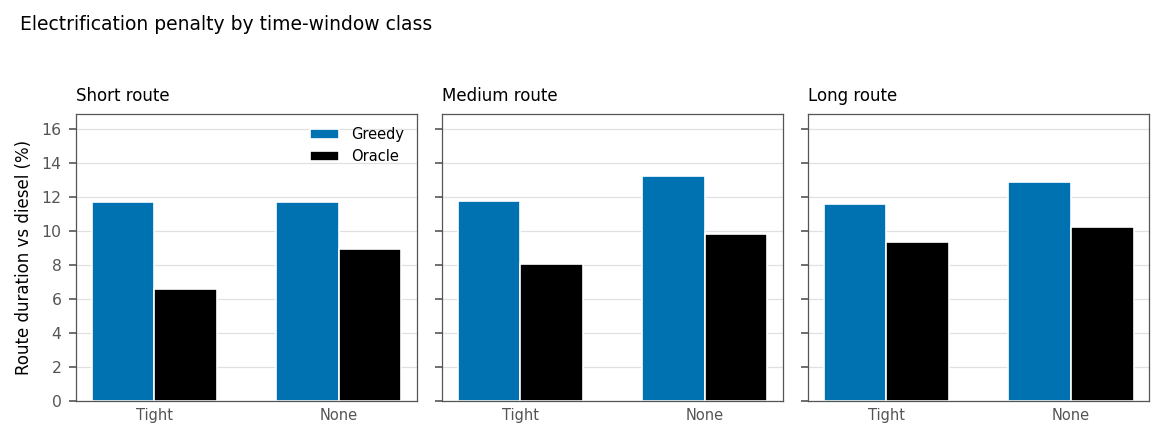
\includegraphics[width=0.85\linewidth]{figures/additional_diesel_tw.png}
    \caption{\red{Electrification penalty by time-window class, duration against objective.}}
    \label{fig:dieseltw}
\end{figure}


\begin{comment}


\section*{CRediT authorship contribution statement}
\noindent
\textbf{Céline Pagnier:} Conceptualization, Methodology, Software, Formal Analysis, Visualization, Writing - original draft.
\textbf{Steffen J. Bakker:} Conceptualization, Methodology, Software, Formal Analysis, Visualization, Writing - original draft.
\textbf{Pernille Seljom:} Conceptualization, Methodology, Software, Writing - Review \& Editing.
\textbf{Asgeir Tomasgard:} Conceptualization, Methodology.


\section*{Acknowledgements}
\noindent
This paper was prepared as a part of the Norwegian Research Centre for Energy
Transition Studies (FME NTRANS, p-nr: 296205), funded by the Research Council of Norway.
\end{comment}


\bibliography{paper4}

\end{document}

\endinput
%%
%% End of file `elsarticle-template-num.tex'.
